\documentclass[twoside]{book}

% Packages required by doxygen
\usepackage{calc}
\usepackage{doxygen}
\usepackage{graphicx}
\usepackage[utf8]{inputenc}
\usepackage{makeidx}
\usepackage{multicol}
\usepackage{multirow}
\usepackage{textcomp}
\usepackage[table]{xcolor}

% Font selection
\usepackage[T1]{fontenc}
\usepackage{mathptmx}
\usepackage[scaled=.90]{helvet}
\usepackage{courier}
\usepackage{amssymb}
\usepackage{sectsty}
\renewcommand{\familydefault}{\sfdefault}
\allsectionsfont{%
  \fontseries{bc}\selectfont%
  \color{darkgray}%
}
\renewcommand{\DoxyLabelFont}{%
  \fontseries{bc}\selectfont%
  \color{darkgray}%
}

% Page & text layout
\usepackage{geometry}
\geometry{%
  a4paper,%
  top=2.5cm,%
  bottom=2.5cm,%
  left=2.5cm,%
  right=2.5cm%
}
\tolerance=750
\hfuzz=15pt
\hbadness=750
\setlength{\emergencystretch}{15pt}
\setlength{\parindent}{0cm}
\setlength{\parskip}{0.2cm}
\makeatletter
\renewcommand{\paragraph}{%
  \@startsection{paragraph}{4}{0ex}{-1.0ex}{1.0ex}{%
    \normalfont\normalsize\bfseries\SS@parafont%
  }%
}
\renewcommand{\subparagraph}{%
  \@startsection{subparagraph}{5}{0ex}{-1.0ex}{1.0ex}{%
    \normalfont\normalsize\bfseries\SS@subparafont%
  }%
}
\makeatother

% Headers & footers
\usepackage{fancyhdr}
\pagestyle{fancyplain}
\fancyhead[LE]{\fancyplain{}{\bfseries\thepage}}
\fancyhead[CE]{\fancyplain{}{}}
\fancyhead[RE]{\fancyplain{}{\bfseries\leftmark}}
\fancyhead[LO]{\fancyplain{}{\bfseries\rightmark}}
\fancyhead[CO]{\fancyplain{}{}}
\fancyhead[RO]{\fancyplain{}{\bfseries\thepage}}
\fancyfoot[LE]{\fancyplain{}{}}
\fancyfoot[CE]{\fancyplain{}{}}
\fancyfoot[RE]{\fancyplain{}{\bfseries\scriptsize Generated on Thu Sep 28 2017 10\-:02\-:03 for Monte\-Carlo\-Pricer by Doxygen }}
\fancyfoot[LO]{\fancyplain{}{\bfseries\scriptsize Generated on Thu Sep 28 2017 10\-:02\-:03 for Monte\-Carlo\-Pricer by Doxygen }}
\fancyfoot[CO]{\fancyplain{}{}}
\fancyfoot[RO]{\fancyplain{}{}}
\renewcommand{\footrulewidth}{0.4pt}
\renewcommand{\chaptermark}[1]{%
  \markboth{#1}{}%
}
\renewcommand{\sectionmark}[1]{%
  \markright{\thesection\ #1}%
}

% Indices & bibliography
\usepackage{natbib}
\usepackage[titles]{tocloft}
\setcounter{tocdepth}{3}
\setcounter{secnumdepth}{5}
\makeindex

% Hyperlinks (required, but should be loaded last)
\usepackage{ifpdf}
\ifpdf
  \usepackage[pdftex,pagebackref=true]{hyperref}
\else
  \usepackage[ps2pdf,pagebackref=true]{hyperref}
\fi
\hypersetup{%
  colorlinks=true,%
  linkcolor=blue,%
  citecolor=blue,%
  unicode%
}

% Custom commands
\newcommand{\clearemptydoublepage}{%
  \newpage{\pagestyle{empty}\cleardoublepage}%
}


%===== C O N T E N T S =====

\begin{document}

% Titlepage & ToC
\hypersetup{pageanchor=false}
\pagenumbering{roman}
\begin{titlepage}
\vspace*{7cm}
\begin{center}%
{\Large Monte\-Carlo\-Pricer \\[1ex]\large 1.\-0 }\\
\vspace*{1cm}
{\large Generated by Doxygen 1.8.5}\\
\vspace*{0.5cm}
{\small Thu Sep 28 2017 10:02:03}\\
\end{center}
\end{titlepage}
\clearemptydoublepage
\tableofcontents
\clearemptydoublepage
\pagenumbering{arabic}
\hypersetup{pageanchor=true}

%--- Begin generated contents ---
\chapter{Hierarchical Index}
\section{Class Hierarchy}
This inheritance list is sorted roughly, but not completely, alphabetically\-:\begin{DoxyCompactList}
\item \contentsline{section}{Black\-Scholes\-Model}{\pageref{classBlackScholesModel}}{}
\item \contentsline{section}{comp}{\pageref{structcomp}}{}
\item \contentsline{section}{Monte\-Carlo}{\pageref{classMonteCarlo}}{}
\item \contentsline{section}{Option}{\pageref{classOption}}{}
\begin{DoxyCompactList}
\item \contentsline{section}{Option\-Asian}{\pageref{classOptionAsian}}{}
\item \contentsline{section}{Option\-Basket}{\pageref{classOptionBasket}}{}
\item \contentsline{section}{Option\-Performance}{\pageref{classOptionPerformance}}{}
\end{DoxyCompactList}
\item \contentsline{section}{Param}{\pageref{classParam}}{}
\begin{DoxyCompactList}
\item \contentsline{section}{Parser}{\pageref{classParser}}{}
\end{DoxyCompactList}
\item \contentsline{section}{Type\-Val}{\pageref{classTypeVal}}{}
\end{DoxyCompactList}

\chapter{Data Structure Index}
\section{Data Structures}
Here are the data structures with brief descriptions\-:\begin{DoxyCompactList}
\item\contentsline{section}{\hyperlink{classBlackScholesModel}{Black\-Scholes\-Model} \\*Modèle de Black Scholes }{\pageref{classBlackScholesModel}}{}
\item\contentsline{section}{\hyperlink{structcomp}{comp} }{\pageref{structcomp}}{}
\item\contentsline{section}{\hyperlink{classMonteCarlo}{Monte\-Carlo} }{\pageref{classMonteCarlo}}{}
\item\contentsline{section}{\hyperlink{classOption}{Option} \\*Classe \hyperlink{classOption}{Option} abstraite }{\pageref{classOption}}{}
\item\contentsline{section}{\hyperlink{classOptionAsian}{Option\-Asian} }{\pageref{classOptionAsian}}{}
\item\contentsline{section}{\hyperlink{classOptionBasket}{Option\-Basket} }{\pageref{classOptionBasket}}{}
\item\contentsline{section}{\hyperlink{classOptionPerformance}{Option\-Performance} }{\pageref{classOptionPerformance}}{}
\item\contentsline{section}{\hyperlink{classParam}{Param} }{\pageref{classParam}}{}
\item\contentsline{section}{\hyperlink{classParser}{Parser} }{\pageref{classParser}}{}
\item\contentsline{section}{\hyperlink{classTypeVal}{Type\-Val} }{\pageref{classTypeVal}}{}
\end{DoxyCompactList}

\chapter{File Index}
\section{File List}
Here is a list of all files with brief descriptions\-:\begin{DoxyCompactList}
\item\contentsline{section}{/user/2/.\-base/margueed/home/pricer\-Monte\-Carlo/src/\hyperlink{BlackScholesModel_8cpp}{Black\-Scholes\-Model.\-cpp} }{\pageref{BlackScholesModel_8cpp}}{}
\item\contentsline{section}{/user/2/.\-base/margueed/home/pricer\-Monte\-Carlo/src/\hyperlink{BlackScholesModel_8hpp}{Black\-Scholes\-Model.\-hpp} }{\pageref{BlackScholesModel_8hpp}}{}
\item\contentsline{section}{/user/2/.\-base/margueed/home/pricer\-Monte\-Carlo/src/\hyperlink{MonteCarlo_8cpp}{Monte\-Carlo.\-cpp} }{\pageref{MonteCarlo_8cpp}}{}
\item\contentsline{section}{/user/2/.\-base/margueed/home/pricer\-Monte\-Carlo/src/\hyperlink{MonteCarlo_8hpp}{Monte\-Carlo.\-hpp} }{\pageref{MonteCarlo_8hpp}}{}
\item\contentsline{section}{/user/2/.\-base/margueed/home/pricer\-Monte\-Carlo/src/\hyperlink{Option_8cpp}{Option.\-cpp} }{\pageref{Option_8cpp}}{}
\item\contentsline{section}{/user/2/.\-base/margueed/home/pricer\-Monte\-Carlo/src/\hyperlink{Option_8hpp}{Option.\-hpp} }{\pageref{Option_8hpp}}{}
\item\contentsline{section}{/user/2/.\-base/margueed/home/pricer\-Monte\-Carlo/src/\hyperlink{OptionAsian_8cpp}{Option\-Asian.\-cpp} }{\pageref{OptionAsian_8cpp}}{}
\item\contentsline{section}{/user/2/.\-base/margueed/home/pricer\-Monte\-Carlo/src/\hyperlink{OptionAsian_8hpp}{Option\-Asian.\-hpp} }{\pageref{OptionAsian_8hpp}}{}
\item\contentsline{section}{/user/2/.\-base/margueed/home/pricer\-Monte\-Carlo/src/\hyperlink{OptionBasket_8cpp}{Option\-Basket.\-cpp} }{\pageref{OptionBasket_8cpp}}{}
\item\contentsline{section}{/user/2/.\-base/margueed/home/pricer\-Monte\-Carlo/src/\hyperlink{OptionBasket_8hpp}{Option\-Basket.\-hpp} }{\pageref{OptionBasket_8hpp}}{}
\item\contentsline{section}{/user/2/.\-base/margueed/home/pricer\-Monte\-Carlo/src/\hyperlink{OptionPerformance_8cpp}{Option\-Performance.\-cpp} }{\pageref{OptionPerformance_8cpp}}{}
\item\contentsline{section}{/user/2/.\-base/margueed/home/pricer\-Monte\-Carlo/src/\hyperlink{OptionPerformance_8hpp}{Option\-Performance.\-hpp} }{\pageref{OptionPerformance_8hpp}}{}
\item\contentsline{section}{/user/2/.\-base/margueed/home/pricer\-Monte\-Carlo/src/\hyperlink{parser_8cpp}{parser.\-cpp} }{\pageref{parser_8cpp}}{}
\item\contentsline{section}{/user/2/.\-base/margueed/home/pricer\-Monte\-Carlo/src/\hyperlink{parser_8hpp}{parser.\-hpp} }{\pageref{parser_8hpp}}{}
\item\contentsline{section}{/user/2/.\-base/margueed/home/pricer\-Monte\-Carlo/src/\hyperlink{Pricer_8cpp}{Pricer.\-cpp} }{\pageref{Pricer_8cpp}}{}
\end{DoxyCompactList}

\chapter{Data Structure Documentation}
\hypertarget{classBlackScholesModel}{\section{Black\-Scholes\-Model Class Reference}
\label{classBlackScholesModel}\index{Black\-Scholes\-Model@{Black\-Scholes\-Model}}
}


Modèle de Black Scholes.  




{\ttfamily \#include $<$Black\-Scholes\-Model.\-hpp$>$}

\subsection*{Public Member Functions}
\begin{DoxyCompactItemize}
\item 
\hyperlink{classBlackScholesModel_abf5c7baafc243266094d4aca57016646}{Black\-Scholes\-Model} (int, double, double, Pnl\-Vect $\ast$, Pnl\-Vect $\ast$, Pnl\-Vect $\ast$)
\begin{DoxyCompactList}\small\item\em valeurs initiales du sous-\/jacent \end{DoxyCompactList}\item 
\hyperlink{classBlackScholesModel_a1f273e39d33b27280f87004c1480635b}{$\sim$\-Black\-Scholes\-Model} ()
\begin{DoxyCompactList}\small\item\em Destructeur de classe. \end{DoxyCompactList}\item 
void \hyperlink{classBlackScholesModel_a71ed54a0ca9a89b87610ff699814e120}{asset} (Pnl\-Mat $\ast$path, double T, int nb\-Time\-Steps, Pnl\-Rng $\ast$rng)
\begin{DoxyCompactList}\small\item\em Génère une trajectoire du modèle et la stocke dans path. \end{DoxyCompactList}\item 
void \hyperlink{classBlackScholesModel_a4ae6f779b9f22255640241e1ed37fbe1}{asset} (Pnl\-Mat $\ast$path, double t, double T, int nb\-Time\-Steps, Pnl\-Rng $\ast$rng, const Pnl\-Mat $\ast$past)
\begin{DoxyCompactList}\small\item\em Calcule une trajectoire du sous-\/jacent connaissant le passé jusqu' à la date t. \end{DoxyCompactList}\item 
void \hyperlink{classBlackScholesModel_ac89a165e6d27cc12dd77627597f7f56d}{shift\-Asset} (Pnl\-Mat $\ast$shift\-\_\-path, const Pnl\-Mat $\ast$path, int d, double h, double t, double timestep)
\begin{DoxyCompactList}\small\item\em Shift d'une trajectoire du sous-\/jacent. \end{DoxyCompactList}\item 
Pnl\-Mat $\ast$ \hyperlink{classBlackScholesModel_a5cefb6798ecf3aad04d7c098846e9381}{simul\-\_\-market} (int H, double T, Pnl\-Rng $\ast$rng)
\begin{DoxyCompactList}\small\item\em Calcule une simulation de marché \end{DoxyCompactList}\item 
void \hyperlink{classBlackScholesModel_ad131019feab3bc199889b840d9d3c7c3}{simul\-\_\-market} (Pnl\-Mat $\ast$path, double T, int H, Pnl\-Rng $\ast$rng)
\end{DoxyCompactItemize}
\subsection*{Data Fields}
\begin{DoxyCompactItemize}
\item 
int \hyperlink{classBlackScholesModel_ab84e9318c0c1e8a50d5e2f9a70f1256e}{size\-\_\-}
\item 
double \hyperlink{classBlackScholesModel_a9b07eb1d8a7ada20e1a723ba19172644}{r\-\_\-}
\begin{DoxyCompactList}\small\item\em nombre d'actifs du modèle \end{DoxyCompactList}\item 
double \hyperlink{classBlackScholesModel_a1022a65929e3656f8990b7b0a63705ba}{rho\-\_\-}
\begin{DoxyCompactList}\small\item\em taux d'intérêt \end{DoxyCompactList}\item 
Pnl\-Vect $\ast$ \hyperlink{classBlackScholesModel_a745a2d85da5056b44bd88f37ee7b33e0}{sigma\-\_\-}
\begin{DoxyCompactList}\small\item\em paramètre de corrélation \end{DoxyCompactList}\item 
Pnl\-Vect $\ast$ \hyperlink{classBlackScholesModel_a6ce6853d5f0d65c8e0f07cdedca3e26a}{spot\-\_\-}
\begin{DoxyCompactList}\small\item\em vecteur de volatilités \end{DoxyCompactList}\end{DoxyCompactItemize}
\subsection*{Protected Attributes}
\begin{DoxyCompactItemize}
\item 
Pnl\-Vect $\ast$ \hyperlink{classBlackScholesModel_af92b535c61f17e7a16af56952739302f}{trend\-\_\-}
\item 
Pnl\-Mat $\ast$ \hyperlink{classBlackScholesModel_a24f36715c6f6b87de76c6fb3067e4e2f}{cholesky}
\begin{DoxyCompactList}\small\item\em Tendance du modèle. \end{DoxyCompactList}\end{DoxyCompactItemize}
\subsection*{Private Attributes}
\begin{DoxyCompactItemize}
\item 
Pnl\-Vect $\ast$ \hyperlink{classBlackScholesModel_ac790e18c09330dc3e62f77e34f3a64a4}{G\-\_\-i}
\begin{DoxyCompactList}\small\item\em Matrice de Cholesky. \end{DoxyCompactList}\item 
Pnl\-Vect $\ast$ \hyperlink{classBlackScholesModel_aae8afe7aed64436e11b245a472135404}{L\-\_\-d}
\item 
Pnl\-Vect $\ast$ \hyperlink{classBlackScholesModel_a28428fd6090bc1062d0ec7612feeaac0}{temp\-Row}
\item 
Pnl\-Vect $\ast$ \hyperlink{classBlackScholesModel_a18801c05f4b88b9cbf39fb48bd8beed4}{spots\-\_\-t}
\end{DoxyCompactItemize}


\subsection{Detailed Description}
Modèle de Black Scholes. 

\subsection{Constructor \& Destructor Documentation}
\hypertarget{classBlackScholesModel_abf5c7baafc243266094d4aca57016646}{\index{Black\-Scholes\-Model@{Black\-Scholes\-Model}!Black\-Scholes\-Model@{Black\-Scholes\-Model}}
\index{Black\-Scholes\-Model@{Black\-Scholes\-Model}!BlackScholesModel@{Black\-Scholes\-Model}}
\subsubsection[{Black\-Scholes\-Model}]{\setlength{\rightskip}{0pt plus 5cm}Black\-Scholes\-Model\-::\-Black\-Scholes\-Model (
\begin{DoxyParamCaption}
\item[{int}]{size, }
\item[{double}]{r, }
\item[{double}]{rho, }
\item[{Pnl\-Vect $\ast$}]{sigma, }
\item[{Pnl\-Vect $\ast$}]{spot, }
\item[{Pnl\-Vect $\ast$}]{trend}
\end{DoxyParamCaption}
)}}\label{classBlackScholesModel_abf5c7baafc243266094d4aca57016646}


valeurs initiales du sous-\/jacent 

Création de la matrice de Cholesky

Création des vecteurs temporaires \hypertarget{classBlackScholesModel_a1f273e39d33b27280f87004c1480635b}{\index{Black\-Scholes\-Model@{Black\-Scholes\-Model}!$\sim$\-Black\-Scholes\-Model@{$\sim$\-Black\-Scholes\-Model}}
\index{$\sim$\-Black\-Scholes\-Model@{$\sim$\-Black\-Scholes\-Model}!BlackScholesModel@{Black\-Scholes\-Model}}
\subsubsection[{$\sim$\-Black\-Scholes\-Model}]{\setlength{\rightskip}{0pt plus 5cm}Black\-Scholes\-Model\-::$\sim$\-Black\-Scholes\-Model (
\begin{DoxyParamCaption}
{}
\end{DoxyParamCaption}
)}}\label{classBlackScholesModel_a1f273e39d33b27280f87004c1480635b}


Destructeur de classe. 

Suppression des vecteurs temporaires 

\subsection{Member Function Documentation}
\hypertarget{classBlackScholesModel_a71ed54a0ca9a89b87610ff699814e120}{\index{Black\-Scholes\-Model@{Black\-Scholes\-Model}!asset@{asset}}
\index{asset@{asset}!BlackScholesModel@{Black\-Scholes\-Model}}
\subsubsection[{asset}]{\setlength{\rightskip}{0pt plus 5cm}void Black\-Scholes\-Model\-::asset (
\begin{DoxyParamCaption}
\item[{Pnl\-Mat $\ast$}]{path, }
\item[{double}]{T, }
\item[{int}]{nb\-Time\-Steps, }
\item[{Pnl\-Rng $\ast$}]{rng}
\end{DoxyParamCaption}
)}}\label{classBlackScholesModel_a71ed54a0ca9a89b87610ff699814e120}


Génère une trajectoire du modèle et la stocke dans path. 


\begin{DoxyParams}[1]{Parameters}
\mbox{\tt out}  & {\em path} & contient une trajectoire du modèle. C'est une matrice de taille (nb\-Time\-Steps+1) x d \\
\hline
\mbox{\tt in}  & {\em T} & maturité \\
\hline
\mbox{\tt in}  & {\em nb\-Time\-Steps} & nombre de dates de constatation \\
\hline
\end{DoxyParams}
Simulation de la trajectoire 

Referenced by Monte\-Carlo\-::delta(), and Monte\-Carlo\-::price().

\hypertarget{classBlackScholesModel_a4ae6f779b9f22255640241e1ed37fbe1}{\index{Black\-Scholes\-Model@{Black\-Scholes\-Model}!asset@{asset}}
\index{asset@{asset}!BlackScholesModel@{Black\-Scholes\-Model}}
\subsubsection[{asset}]{\setlength{\rightskip}{0pt plus 5cm}void Black\-Scholes\-Model\-::asset (
\begin{DoxyParamCaption}
\item[{Pnl\-Mat $\ast$}]{path, }
\item[{double}]{t, }
\item[{double}]{T, }
\item[{int}]{nb\-Time\-Steps, }
\item[{Pnl\-Rng $\ast$}]{rng, }
\item[{const Pnl\-Mat $\ast$}]{past}
\end{DoxyParamCaption}
)}}\label{classBlackScholesModel_a4ae6f779b9f22255640241e1ed37fbe1}


Calcule une trajectoire du sous-\/jacent connaissant le passé jusqu' à la date t. 


\begin{DoxyParams}[1]{Parameters}
\mbox{\tt out}  & {\em path} & contient une trajectoire du sous-\/jacent donnée jusqu'à l'instant t par la matrice past \\
\hline
\mbox{\tt in}  & {\em t} & date jusqu'à laquelle on connait la trajectoire. t n'est pas forcément une date de discrétisation \\
\hline
\mbox{\tt in}  & {\em nb\-Time\-Steps} & nombre de pas de constatation \\
\hline
\mbox{\tt in}  & {\em T} & date jusqu'à laquelle on simule la trajectoire \\
\hline
\mbox{\tt in}  & {\em past} & trajectoire réalisée jusqu'a la date t \\
\hline
\end{DoxyParams}
Copie de la trajectoire passée dans la trajectoire totale

Sauvegarde des spots

Simulation de la trajectoire \hypertarget{classBlackScholesModel_ac89a165e6d27cc12dd77627597f7f56d}{\index{Black\-Scholes\-Model@{Black\-Scholes\-Model}!shift\-Asset@{shift\-Asset}}
\index{shift\-Asset@{shift\-Asset}!BlackScholesModel@{Black\-Scholes\-Model}}
\subsubsection[{shift\-Asset}]{\setlength{\rightskip}{0pt plus 5cm}void Black\-Scholes\-Model\-::shift\-Asset (
\begin{DoxyParamCaption}
\item[{Pnl\-Mat $\ast$}]{shift\-\_\-path, }
\item[{const Pnl\-Mat $\ast$}]{path, }
\item[{int}]{d, }
\item[{double}]{h, }
\item[{double}]{t, }
\item[{double}]{timestep}
\end{DoxyParamCaption}
)}}\label{classBlackScholesModel_ac89a165e6d27cc12dd77627597f7f56d}


Shift d'une trajectoire du sous-\/jacent. 


\begin{DoxyParams}[1]{Parameters}
\mbox{\tt in}  & {\em path} & contient en input la trajectoire du sous-\/jacent \\
\hline
\mbox{\tt out}  & {\em shift\-\_\-path} & contient la trajectoire path dont la composante d a été shiftée par (1+h) à partir de la date t. \\
\hline
\mbox{\tt in}  & {\em t} & date à partir de laquelle on shift \\
\hline
\mbox{\tt in}  & {\em h} & pas de différences finies \\
\hline
\mbox{\tt in}  & {\em d} & indice du sous-\/jacent à shifter \\
\hline
\mbox{\tt in}  & {\em timestep} & pas de constatation du sous-\/jacent \\
\hline
\end{DoxyParams}


Referenced by Monte\-Carlo\-::delta().

\hypertarget{classBlackScholesModel_a5cefb6798ecf3aad04d7c098846e9381}{\index{Black\-Scholes\-Model@{Black\-Scholes\-Model}!simul\-\_\-market@{simul\-\_\-market}}
\index{simul\-\_\-market@{simul\-\_\-market}!BlackScholesModel@{Black\-Scholes\-Model}}
\subsubsection[{simul\-\_\-market}]{\setlength{\rightskip}{0pt plus 5cm}Pnl\-Mat $\ast$ Black\-Scholes\-Model\-::simul\-\_\-market (
\begin{DoxyParamCaption}
\item[{int}]{H, }
\item[{double}]{T, }
\item[{Pnl\-Rng $\ast$}]{rng}
\end{DoxyParamCaption}
)}}\label{classBlackScholesModel_a5cefb6798ecf3aad04d7c098846e9381}


Calcule une simulation de marché 


\begin{DoxyParams}[1]{Parameters}
\mbox{\tt in}  & {\em H} & le nombre de dates \\
\hline
\mbox{\tt in}  & {\em T} & la maturité \\
\hline
\mbox{\tt in}  & {\em rng} & le générateur aléatoire \\
\hline
\end{DoxyParams}
Simulation de la trajectoire 

Referenced by main().

\hypertarget{classBlackScholesModel_ad131019feab3bc199889b840d9d3c7c3}{\index{Black\-Scholes\-Model@{Black\-Scholes\-Model}!simul\-\_\-market@{simul\-\_\-market}}
\index{simul\-\_\-market@{simul\-\_\-market}!BlackScholesModel@{Black\-Scholes\-Model}}
\subsubsection[{simul\-\_\-market}]{\setlength{\rightskip}{0pt plus 5cm}void Black\-Scholes\-Model\-::simul\-\_\-market (
\begin{DoxyParamCaption}
\item[{Pnl\-Mat $\ast$}]{path, }
\item[{double}]{T, }
\item[{int}]{H, }
\item[{Pnl\-Rng $\ast$}]{rng}
\end{DoxyParamCaption}
)}}\label{classBlackScholesModel_ad131019feab3bc199889b840d9d3c7c3}


\subsection{Field Documentation}
\hypertarget{classBlackScholesModel_a24f36715c6f6b87de76c6fb3067e4e2f}{\index{Black\-Scholes\-Model@{Black\-Scholes\-Model}!cholesky@{cholesky}}
\index{cholesky@{cholesky}!BlackScholesModel@{Black\-Scholes\-Model}}
\subsubsection[{cholesky}]{\setlength{\rightskip}{0pt plus 5cm}Pnl\-Mat$\ast$ Black\-Scholes\-Model\-::cholesky\hspace{0.3cm}{\ttfamily [protected]}}}\label{classBlackScholesModel_a24f36715c6f6b87de76c6fb3067e4e2f}


Tendance du modèle. 

\hypertarget{classBlackScholesModel_ac790e18c09330dc3e62f77e34f3a64a4}{\index{Black\-Scholes\-Model@{Black\-Scholes\-Model}!G\-\_\-i@{G\-\_\-i}}
\index{G\-\_\-i@{G\-\_\-i}!BlackScholesModel@{Black\-Scholes\-Model}}
\subsubsection[{G\-\_\-i}]{\setlength{\rightskip}{0pt plus 5cm}Pnl\-Vect$\ast$ Black\-Scholes\-Model\-::\-G\-\_\-i\hspace{0.3cm}{\ttfamily [private]}}}\label{classBlackScholesModel_ac790e18c09330dc3e62f77e34f3a64a4}


Matrice de Cholesky. 

Déclaration ici afin de limiter les créations et suppressions à chaque appel \hypertarget{classBlackScholesModel_aae8afe7aed64436e11b245a472135404}{\index{Black\-Scholes\-Model@{Black\-Scholes\-Model}!L\-\_\-d@{L\-\_\-d}}
\index{L\-\_\-d@{L\-\_\-d}!BlackScholesModel@{Black\-Scholes\-Model}}
\subsubsection[{L\-\_\-d}]{\setlength{\rightskip}{0pt plus 5cm}Pnl\-Vect$\ast$ Black\-Scholes\-Model\-::\-L\-\_\-d\hspace{0.3cm}{\ttfamily [private]}}}\label{classBlackScholesModel_aae8afe7aed64436e11b245a472135404}
\hypertarget{classBlackScholesModel_a9b07eb1d8a7ada20e1a723ba19172644}{\index{Black\-Scholes\-Model@{Black\-Scholes\-Model}!r\-\_\-@{r\-\_\-}}
\index{r\-\_\-@{r\-\_\-}!BlackScholesModel@{Black\-Scholes\-Model}}
\subsubsection[{r\-\_\-}]{\setlength{\rightskip}{0pt plus 5cm}double Black\-Scholes\-Model\-::r\-\_\-}}\label{classBlackScholesModel_a9b07eb1d8a7ada20e1a723ba19172644}


nombre d'actifs du modèle 



Referenced by Monte\-Carlo\-::delta(), Monte\-Carlo\-::hedging\-P\-And\-L(), and Monte\-Carlo\-::price().

\hypertarget{classBlackScholesModel_a1022a65929e3656f8990b7b0a63705ba}{\index{Black\-Scholes\-Model@{Black\-Scholes\-Model}!rho\-\_\-@{rho\-\_\-}}
\index{rho\-\_\-@{rho\-\_\-}!BlackScholesModel@{Black\-Scholes\-Model}}
\subsubsection[{rho\-\_\-}]{\setlength{\rightskip}{0pt plus 5cm}double Black\-Scholes\-Model\-::rho\-\_\-}}\label{classBlackScholesModel_a1022a65929e3656f8990b7b0a63705ba}


taux d'intérêt 

\hypertarget{classBlackScholesModel_a745a2d85da5056b44bd88f37ee7b33e0}{\index{Black\-Scholes\-Model@{Black\-Scholes\-Model}!sigma\-\_\-@{sigma\-\_\-}}
\index{sigma\-\_\-@{sigma\-\_\-}!BlackScholesModel@{Black\-Scholes\-Model}}
\subsubsection[{sigma\-\_\-}]{\setlength{\rightskip}{0pt plus 5cm}Pnl\-Vect$\ast$ Black\-Scholes\-Model\-::sigma\-\_\-}}\label{classBlackScholesModel_a745a2d85da5056b44bd88f37ee7b33e0}


paramètre de corrélation 

\hypertarget{classBlackScholesModel_ab84e9318c0c1e8a50d5e2f9a70f1256e}{\index{Black\-Scholes\-Model@{Black\-Scholes\-Model}!size\-\_\-@{size\-\_\-}}
\index{size\-\_\-@{size\-\_\-}!BlackScholesModel@{Black\-Scholes\-Model}}
\subsubsection[{size\-\_\-}]{\setlength{\rightskip}{0pt plus 5cm}int Black\-Scholes\-Model\-::size\-\_\-}}\label{classBlackScholesModel_ab84e9318c0c1e8a50d5e2f9a70f1256e}


Referenced by Monte\-Carlo\-::delta(), Monte\-Carlo\-::hedging\-P\-And\-L(), and Monte\-Carlo\-::\-Monte\-Carlo().

\hypertarget{classBlackScholesModel_a6ce6853d5f0d65c8e0f07cdedca3e26a}{\index{Black\-Scholes\-Model@{Black\-Scholes\-Model}!spot\-\_\-@{spot\-\_\-}}
\index{spot\-\_\-@{spot\-\_\-}!BlackScholesModel@{Black\-Scholes\-Model}}
\subsubsection[{spot\-\_\-}]{\setlength{\rightskip}{0pt plus 5cm}Pnl\-Vect$\ast$ Black\-Scholes\-Model\-::spot\-\_\-}}\label{classBlackScholesModel_a6ce6853d5f0d65c8e0f07cdedca3e26a}


vecteur de volatilités 

\hypertarget{classBlackScholesModel_a18801c05f4b88b9cbf39fb48bd8beed4}{\index{Black\-Scholes\-Model@{Black\-Scholes\-Model}!spots\-\_\-t@{spots\-\_\-t}}
\index{spots\-\_\-t@{spots\-\_\-t}!BlackScholesModel@{Black\-Scholes\-Model}}
\subsubsection[{spots\-\_\-t}]{\setlength{\rightskip}{0pt plus 5cm}Pnl\-Vect$\ast$ Black\-Scholes\-Model\-::spots\-\_\-t\hspace{0.3cm}{\ttfamily [private]}}}\label{classBlackScholesModel_a18801c05f4b88b9cbf39fb48bd8beed4}
\hypertarget{classBlackScholesModel_a28428fd6090bc1062d0ec7612feeaac0}{\index{Black\-Scholes\-Model@{Black\-Scholes\-Model}!temp\-Row@{temp\-Row}}
\index{temp\-Row@{temp\-Row}!BlackScholesModel@{Black\-Scholes\-Model}}
\subsubsection[{temp\-Row}]{\setlength{\rightskip}{0pt plus 5cm}Pnl\-Vect$\ast$ Black\-Scholes\-Model\-::temp\-Row\hspace{0.3cm}{\ttfamily [private]}}}\label{classBlackScholesModel_a28428fd6090bc1062d0ec7612feeaac0}
\hypertarget{classBlackScholesModel_af92b535c61f17e7a16af56952739302f}{\index{Black\-Scholes\-Model@{Black\-Scholes\-Model}!trend\-\_\-@{trend\-\_\-}}
\index{trend\-\_\-@{trend\-\_\-}!BlackScholesModel@{Black\-Scholes\-Model}}
\subsubsection[{trend\-\_\-}]{\setlength{\rightskip}{0pt plus 5cm}Pnl\-Vect$\ast$ Black\-Scholes\-Model\-::trend\-\_\-\hspace{0.3cm}{\ttfamily [protected]}}}\label{classBlackScholesModel_af92b535c61f17e7a16af56952739302f}


The documentation for this class was generated from the following files\-:\begin{DoxyCompactItemize}
\item 
/user/0/.\-base/charmont/home/\-Documents/3\-A/\-Projet/pricer\-Monte\-Carlo/src/\hyperlink{BlackScholesModel_8hpp}{Black\-Scholes\-Model.\-hpp}\item 
/user/0/.\-base/charmont/home/\-Documents/3\-A/\-Projet/pricer\-Monte\-Carlo/src/\hyperlink{BlackScholesModel_8cpp}{Black\-Scholes\-Model.\-cpp}\end{DoxyCompactItemize}

\hypertarget{structcomp}{\section{comp Struct Reference}
\label{structcomp}\index{comp@{comp}}
}


{\ttfamily \#include $<$parser.\-hpp$>$}

\subsection*{Public Member Functions}
\begin{DoxyCompactItemize}
\item 
bool \hyperlink{structcomp_a2c7d3d9dc2c7299c133860001e327f99}{operator()} (const std\-::string \&lhs, const std\-::string \&rhs) const 
\end{DoxyCompactItemize}


\subsection{Member Function Documentation}
\hypertarget{structcomp_a2c7d3d9dc2c7299c133860001e327f99}{\index{comp@{comp}!operator()@{operator()}}
\index{operator()@{operator()}!comp@{comp}}
\subsubsection[{operator()}]{\setlength{\rightskip}{0pt plus 5cm}bool comp\-::operator() (
\begin{DoxyParamCaption}
\item[{const std\-::string \&}]{lhs, }
\item[{const std\-::string \&}]{rhs}
\end{DoxyParamCaption}
) const\hspace{0.3cm}{\ttfamily [inline]}}}\label{structcomp_a2c7d3d9dc2c7299c133860001e327f99}


The documentation for this struct was generated from the following file\-:\begin{DoxyCompactItemize}
\item 
/user/0/.\-base/charmont/home/\-Documents/3\-A/\-Projet/pricer\-Monte\-Carlo/src/\hyperlink{parser_8hpp}{parser.\-hpp}\end{DoxyCompactItemize}

\hypertarget{classMonteCarlo}{\section{Monte\-Carlo Class Reference}
\label{classMonteCarlo}\index{Monte\-Carlo@{Monte\-Carlo}}
}


{\ttfamily \#include $<$Monte\-Carlo.\-hpp$>$}



Collaboration diagram for Monte\-Carlo\-:\nopagebreak
\begin{figure}[H]
\begin{center}
\leavevmode
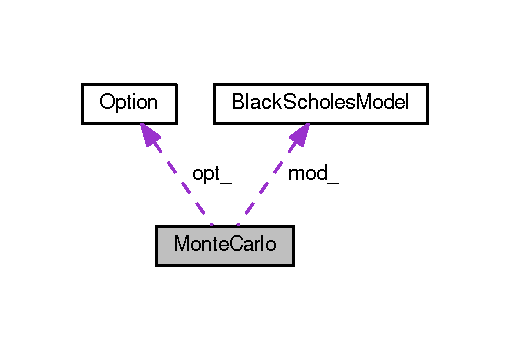
\includegraphics[width=245pt]{classMonteCarlo__coll__graph}
\end{center}
\end{figure}
\subsection*{Public Member Functions}
\begin{DoxyCompactItemize}
\item 
\hyperlink{classMonteCarlo_a01b66bd9e983f9adc235bd80c1c544bd}{Monte\-Carlo} (\hyperlink{classBlackScholesModel}{Black\-Scholes\-Model} $\ast$mod, \hyperlink{classOption}{Option} $\ast$opt, Pnl\-Rng $\ast$rng, double fd\-Step, int nb\-Samples)
\begin{DoxyCompactList}\small\item\em Constructeur de la classe. \end{DoxyCompactList}\item 
\hyperlink{classMonteCarlo_af53fc3a679af18b51a3002b4c1f6b6c2}{$\sim$\-Monte\-Carlo} ()
\begin{DoxyCompactList}\small\item\em Destructeur de classe. \end{DoxyCompactList}\item 
void \hyperlink{classMonteCarlo_a5979d4378e3f28878152a310d8a1f7bf}{price} (double \&prix, double \&ic)
\begin{DoxyCompactList}\small\item\em Calcule le prix de l'option à la date 0. \end{DoxyCompactList}\item 
void \hyperlink{classMonteCarlo_aa7bfce4384323c697d0b06840ad3140f}{price} (const Pnl\-Mat $\ast$past, double t, double \&prix, double \&ic)
\begin{DoxyCompactList}\small\item\em Calcule le prix de l'option à la date t. \end{DoxyCompactList}\item 
void \hyperlink{classMonteCarlo_a340cd456dbe44df20cbc44d40c4df5f5}{delta} (const Pnl\-Mat $\ast$past, double t, Pnl\-Vect $\ast$delta)
\begin{DoxyCompactList}\small\item\em Calcule le delta de l'option à la date t. \end{DoxyCompactList}\item 
double \hyperlink{classMonteCarlo_a24bfcbce4eabfc4382c194139cd7893b}{hedging\-P\-And\-L} (Pnl\-Vect $\ast$result, Pnl\-Mat $\ast$\hyperlink{classMonteCarlo_acf1971465a6503457dfacd397f29ee89}{path}, int H)
\begin{DoxyCompactList}\small\item\em Calcule le profit\&loss du portefeuille de couverture. \end{DoxyCompactList}\end{DoxyCompactItemize}
\subsection*{Data Fields}
\begin{DoxyCompactItemize}
\item 
\hyperlink{classBlackScholesModel}{Black\-Scholes\-Model} $\ast$ \hyperlink{classMonteCarlo_a704c29cd8aa027ab01cc556d37c9a764}{mod\-\_\-}
\item 
\hyperlink{classOption}{Option} $\ast$ \hyperlink{classMonteCarlo_af0ee580b0eb87f57c7a41cd2a9e6fc6a}{opt\-\_\-}
\item 
Pnl\-Rng $\ast$ \hyperlink{classMonteCarlo_aa41318b565311457e04383047d68936e}{rng\-\_\-}
\item 
double \hyperlink{classMonteCarlo_a87640dad0fffa3c38d70c8be6c8d61cb}{fd\-Step\-\_\-}
\item 
int \hyperlink{classMonteCarlo_a82f5bfded3f8b62f22afaa50f7e73ffe}{nb\-Samples\-\_\-}
\end{DoxyCompactItemize}
\subsection*{Private Attributes}
\begin{DoxyCompactItemize}
\item 
Pnl\-Mat $\ast$ \hyperlink{classMonteCarlo_a713c3dd7942f90fde1b0d9d115733580}{spots\-Mat}
\item 
Pnl\-Mat $\ast$ \hyperlink{classMonteCarlo_a07755948492ef0832d5e131c1f010565}{shift\-\_\-path}
\item 
Pnl\-Mat $\ast$ \hyperlink{classMonteCarlo_acf1971465a6503457dfacd397f29ee89}{path}
\end{DoxyCompactItemize}


\subsection{Constructor \& Destructor Documentation}
\hypertarget{classMonteCarlo_a01b66bd9e983f9adc235bd80c1c544bd}{\index{Monte\-Carlo@{Monte\-Carlo}!Monte\-Carlo@{Monte\-Carlo}}
\index{Monte\-Carlo@{Monte\-Carlo}!MonteCarlo@{Monte\-Carlo}}
\subsubsection[{Monte\-Carlo}]{\setlength{\rightskip}{0pt plus 5cm}Monte\-Carlo\-::\-Monte\-Carlo (
\begin{DoxyParamCaption}
\item[{{\bf Black\-Scholes\-Model} $\ast$}]{mod, }
\item[{{\bf Option} $\ast$}]{opt, }
\item[{Pnl\-Rng $\ast$}]{rng, }
\item[{double}]{fd\-Step, }
\item[{int}]{nb\-Samples}
\end{DoxyParamCaption}
)}}\label{classMonteCarlo_a01b66bd9e983f9adc235bd80c1c544bd}


Constructeur de la classe. 

nombre de tirages Monte Carlo
\begin{DoxyParams}[1]{Parameters}
\mbox{\tt in}  & {\em modele} & Black Scholes \\
\hline
\mbox{\tt in}  & {\em l'option} & \\
\hline
\mbox{\tt in}  & {\em le} & générateur \\
\hline
\mbox{\tt in}  & {\em pas} & de différence finie \\
\hline
\mbox{\tt in}  & {\em nombre} & de tirages Monte Carlo \\
\hline
\end{DoxyParams}
Initialisation des variables temporaires 

References fd\-Step\-\_\-, mod\-\_\-, nb\-Samples\-\_\-, Option\-::nb\-Time\-Steps\-\_\-, opt\-\_\-, path, rng\-\_\-, shift\-\_\-path, Black\-Scholes\-Model\-::size\-\_\-, and spots\-Mat.

\hypertarget{classMonteCarlo_af53fc3a679af18b51a3002b4c1f6b6c2}{\index{Monte\-Carlo@{Monte\-Carlo}!$\sim$\-Monte\-Carlo@{$\sim$\-Monte\-Carlo}}
\index{$\sim$\-Monte\-Carlo@{$\sim$\-Monte\-Carlo}!MonteCarlo@{Monte\-Carlo}}
\subsubsection[{$\sim$\-Monte\-Carlo}]{\setlength{\rightskip}{0pt plus 5cm}Monte\-Carlo\-::$\sim$\-Monte\-Carlo (
\begin{DoxyParamCaption}
{}
\end{DoxyParamCaption}
)}}\label{classMonteCarlo_af53fc3a679af18b51a3002b4c1f6b6c2}


Destructeur de classe. 



References path, shift\-\_\-path, and spots\-Mat.



\subsection{Member Function Documentation}
\hypertarget{classMonteCarlo_a340cd456dbe44df20cbc44d40c4df5f5}{\index{Monte\-Carlo@{Monte\-Carlo}!delta@{delta}}
\index{delta@{delta}!MonteCarlo@{Monte\-Carlo}}
\subsubsection[{delta}]{\setlength{\rightskip}{0pt plus 5cm}void Monte\-Carlo\-::delta (
\begin{DoxyParamCaption}
\item[{const Pnl\-Mat $\ast$}]{past, }
\item[{double}]{t, }
\item[{Pnl\-Vect $\ast$}]{delta}
\end{DoxyParamCaption}
)}}\label{classMonteCarlo_a340cd456dbe44df20cbc44d40c4df5f5}


Calcule le delta de l'option à la date t. 


\begin{DoxyParams}[1]{Parameters}
\mbox{\tt in}  & {\em past} & contient la trajectoire du sous-\/jacent jusqu'à l'instant t \\
\hline
\mbox{\tt in}  & {\em t} & date à laquelle le calcul est fait \\
\hline
\mbox{\tt out}  & {\em delta} & contient le vecteur de delta de confiance sur le calcul du delta \\
\hline
\end{DoxyParams}


References Black\-Scholes\-Model\-::asset(), fd\-Step\-\_\-, mod\-\_\-, nb\-Samples\-\_\-, Option\-::nb\-Time\-Steps\-\_\-, opt\-\_\-, path, Option\-::payoff(), Black\-Scholes\-Model\-::r\-\_\-, rng\-\_\-, shift\-\_\-path, Black\-Scholes\-Model\-::shift\-Asset(), Black\-Scholes\-Model\-::size\-\_\-, and Option\-::\-T\-\_\-.



Referenced by hedging\-P\-And\-L(), and main().

\hypertarget{classMonteCarlo_a24bfcbce4eabfc4382c194139cd7893b}{\index{Monte\-Carlo@{Monte\-Carlo}!hedging\-P\-And\-L@{hedging\-P\-And\-L}}
\index{hedging\-P\-And\-L@{hedging\-P\-And\-L}!MonteCarlo@{Monte\-Carlo}}
\subsubsection[{hedging\-P\-And\-L}]{\setlength{\rightskip}{0pt plus 5cm}double Monte\-Carlo\-::hedging\-P\-And\-L (
\begin{DoxyParamCaption}
\item[{Pnl\-Vect $\ast$}]{result, }
\item[{Pnl\-Mat $\ast$}]{path, }
\item[{int}]{H}
\end{DoxyParamCaption}
)}}\label{classMonteCarlo_a24bfcbce4eabfc4382c194139cd7893b}


Calcule le profit\&loss du portefeuille de couverture. 


\begin{DoxyParams}[1]{Parameters}
\mbox{\tt out}  & {\em result} & contient les profit\&loss du portefeuille au cours de la trajectoire \\
\hline
\mbox{\tt in}  & {\em path} & contient la trajectoire des sous-\/jacents \\
\hline
\end{DoxyParams}
\begin{DoxyReturn}{Returns}
le profit\&loss final du portefeuille de couverture 
\end{DoxyReturn}
Initialisation

Calcul du prix initial de l'option

Calcul des deltas initiaux

Complétion de la matrice result

Free the memory 

References delta(), mod\-\_\-, Option\-::nb\-Time\-Steps\-\_\-, opt\-\_\-, Option\-::payoff(), price(), Black\-Scholes\-Model\-::r\-\_\-, Black\-Scholes\-Model\-::size\-\_\-, and Option\-::\-T\-\_\-.



Referenced by main().

\hypertarget{classMonteCarlo_a5979d4378e3f28878152a310d8a1f7bf}{\index{Monte\-Carlo@{Monte\-Carlo}!price@{price}}
\index{price@{price}!MonteCarlo@{Monte\-Carlo}}
\subsubsection[{price}]{\setlength{\rightskip}{0pt plus 5cm}void Monte\-Carlo\-::price (
\begin{DoxyParamCaption}
\item[{double \&}]{prix, }
\item[{double \&}]{ic}
\end{DoxyParamCaption}
)}}\label{classMonteCarlo_a5979d4378e3f28878152a310d8a1f7bf}


Calcule le prix de l'option à la date 0. 


\begin{DoxyParams}[1]{Parameters}
\mbox{\tt out}  & {\em prix} & valeur de l'estimateur Monte Carlo \\
\hline
\mbox{\tt out}  & {\em ic} & largeur de l'intervalle de confiance \\
\hline
\end{DoxyParams}
Calcul du prix

Confidence interval in 95\% 

References Black\-Scholes\-Model\-::asset(), mod\-\_\-, nb\-Samples\-\_\-, Option\-::nb\-Time\-Steps\-\_\-, opt\-\_\-, Option\-::payoff(), Black\-Scholes\-Model\-::r\-\_\-, rng\-\_\-, spots\-Mat, and Option\-::\-T\-\_\-.



Referenced by hedging\-P\-And\-L(), and main().

\hypertarget{classMonteCarlo_aa7bfce4384323c697d0b06840ad3140f}{\index{Monte\-Carlo@{Monte\-Carlo}!price@{price}}
\index{price@{price}!MonteCarlo@{Monte\-Carlo}}
\subsubsection[{price}]{\setlength{\rightskip}{0pt plus 5cm}void Monte\-Carlo\-::price (
\begin{DoxyParamCaption}
\item[{const Pnl\-Mat $\ast$}]{past, }
\item[{double}]{t, }
\item[{double \&}]{prix, }
\item[{double \&}]{ic}
\end{DoxyParamCaption}
)}}\label{classMonteCarlo_aa7bfce4384323c697d0b06840ad3140f}


Calcule le prix de l'option à la date t. 


\begin{DoxyParams}[1]{Parameters}
\mbox{\tt in}  & {\em past} & contient la trajectoire du sous-\/jacent jusqu'à l'instant t \\
\hline
\mbox{\tt in}  & {\em t} & date à laquelle le calcul est fait \\
\hline
\mbox{\tt out}  & {\em prix} & contient le prix \\
\hline
\mbox{\tt out}  & {\em ic} & contient la largeur de l'intervalle de confiance sur le calcul du prix \\
\hline
\end{DoxyParams}
Price computing

Confidence interval in 95\% 

References Black\-Scholes\-Model\-::asset(), mod\-\_\-, nb\-Samples\-\_\-, Option\-::nb\-Time\-Steps\-\_\-, opt\-\_\-, Option\-::payoff(), Black\-Scholes\-Model\-::r\-\_\-, rng\-\_\-, spots\-Mat, and Option\-::\-T\-\_\-.



\subsection{Field Documentation}
\hypertarget{classMonteCarlo_a87640dad0fffa3c38d70c8be6c8d61cb}{\index{Monte\-Carlo@{Monte\-Carlo}!fd\-Step\-\_\-@{fd\-Step\-\_\-}}
\index{fd\-Step\-\_\-@{fd\-Step\-\_\-}!MonteCarlo@{Monte\-Carlo}}
\subsubsection[{fd\-Step\-\_\-}]{\setlength{\rightskip}{0pt plus 5cm}double Monte\-Carlo\-::fd\-Step\-\_\-}}\label{classMonteCarlo_a87640dad0fffa3c38d70c8be6c8d61cb}
pointeur sur le générateur 

Referenced by delta(), and Monte\-Carlo().

\hypertarget{classMonteCarlo_a704c29cd8aa027ab01cc556d37c9a764}{\index{Monte\-Carlo@{Monte\-Carlo}!mod\-\_\-@{mod\-\_\-}}
\index{mod\-\_\-@{mod\-\_\-}!MonteCarlo@{Monte\-Carlo}}
\subsubsection[{mod\-\_\-}]{\setlength{\rightskip}{0pt plus 5cm}{\bf Black\-Scholes\-Model}$\ast$ Monte\-Carlo\-::mod\-\_\-}}\label{classMonteCarlo_a704c29cd8aa027ab01cc556d37c9a764}


Referenced by delta(), hedging\-P\-And\-L(), Monte\-Carlo(), and price().

\hypertarget{classMonteCarlo_a82f5bfded3f8b62f22afaa50f7e73ffe}{\index{Monte\-Carlo@{Monte\-Carlo}!nb\-Samples\-\_\-@{nb\-Samples\-\_\-}}
\index{nb\-Samples\-\_\-@{nb\-Samples\-\_\-}!MonteCarlo@{Monte\-Carlo}}
\subsubsection[{nb\-Samples\-\_\-}]{\setlength{\rightskip}{0pt plus 5cm}int Monte\-Carlo\-::nb\-Samples\-\_\-}}\label{classMonteCarlo_a82f5bfded3f8b62f22afaa50f7e73ffe}
pas de différence finie 

Referenced by delta(), Monte\-Carlo(), and price().

\hypertarget{classMonteCarlo_af0ee580b0eb87f57c7a41cd2a9e6fc6a}{\index{Monte\-Carlo@{Monte\-Carlo}!opt\-\_\-@{opt\-\_\-}}
\index{opt\-\_\-@{opt\-\_\-}!MonteCarlo@{Monte\-Carlo}}
\subsubsection[{opt\-\_\-}]{\setlength{\rightskip}{0pt plus 5cm}{\bf Option}$\ast$ Monte\-Carlo\-::opt\-\_\-}}\label{classMonteCarlo_af0ee580b0eb87f57c7a41cd2a9e6fc6a}
pointeur vers le modèle 

Referenced by delta(), hedging\-P\-And\-L(), Monte\-Carlo(), and price().

\hypertarget{classMonteCarlo_acf1971465a6503457dfacd397f29ee89}{\index{Monte\-Carlo@{Monte\-Carlo}!path@{path}}
\index{path@{path}!MonteCarlo@{Monte\-Carlo}}
\subsubsection[{path}]{\setlength{\rightskip}{0pt plus 5cm}Pnl\-Mat$\ast$ Monte\-Carlo\-::path\hspace{0.3cm}{\ttfamily [private]}}}\label{classMonteCarlo_acf1971465a6503457dfacd397f29ee89}


Referenced by delta(), Monte\-Carlo(), and $\sim$\-Monte\-Carlo().

\hypertarget{classMonteCarlo_aa41318b565311457e04383047d68936e}{\index{Monte\-Carlo@{Monte\-Carlo}!rng\-\_\-@{rng\-\_\-}}
\index{rng\-\_\-@{rng\-\_\-}!MonteCarlo@{Monte\-Carlo}}
\subsubsection[{rng\-\_\-}]{\setlength{\rightskip}{0pt plus 5cm}Pnl\-Rng$\ast$ Monte\-Carlo\-::rng\-\_\-}}\label{classMonteCarlo_aa41318b565311457e04383047d68936e}
pointeur sur l'option 

Referenced by delta(), Monte\-Carlo(), and price().

\hypertarget{classMonteCarlo_a07755948492ef0832d5e131c1f010565}{\index{Monte\-Carlo@{Monte\-Carlo}!shift\-\_\-path@{shift\-\_\-path}}
\index{shift\-\_\-path@{shift\-\_\-path}!MonteCarlo@{Monte\-Carlo}}
\subsubsection[{shift\-\_\-path}]{\setlength{\rightskip}{0pt plus 5cm}Pnl\-Mat$\ast$ Monte\-Carlo\-::shift\-\_\-path\hspace{0.3cm}{\ttfamily [private]}}}\label{classMonteCarlo_a07755948492ef0832d5e131c1f010565}


Referenced by delta(), Monte\-Carlo(), and $\sim$\-Monte\-Carlo().

\hypertarget{classMonteCarlo_a713c3dd7942f90fde1b0d9d115733580}{\index{Monte\-Carlo@{Monte\-Carlo}!spots\-Mat@{spots\-Mat}}
\index{spots\-Mat@{spots\-Mat}!MonteCarlo@{Monte\-Carlo}}
\subsubsection[{spots\-Mat}]{\setlength{\rightskip}{0pt plus 5cm}Pnl\-Mat$\ast$ Monte\-Carlo\-::spots\-Mat\hspace{0.3cm}{\ttfamily [private]}}}\label{classMonteCarlo_a713c3dd7942f90fde1b0d9d115733580}


Referenced by Monte\-Carlo(), price(), and $\sim$\-Monte\-Carlo().



The documentation for this class was generated from the following files\-:\begin{DoxyCompactItemize}
\item 
/user/0/.\-base/charmont/home/\-Documents/3\-A/\-Projet/pricer\-Monte\-Carlo/src/\hyperlink{MonteCarlo_8hpp}{Monte\-Carlo.\-hpp}\item 
/user/0/.\-base/charmont/home/\-Documents/3\-A/\-Projet/pricer\-Monte\-Carlo/src/\hyperlink{MonteCarlo_8cpp}{Monte\-Carlo.\-cpp}\end{DoxyCompactItemize}

\hypertarget{classOption}{\section{Option Class Reference}
\label{classOption}\index{Option@{Option}}
}


Classe \hyperlink{classOption}{Option} abstraite.  




{\ttfamily \#include $<$Option.\-hpp$>$}



Inheritance diagram for Option\-:\nopagebreak
\begin{figure}[H]
\begin{center}
\leavevmode
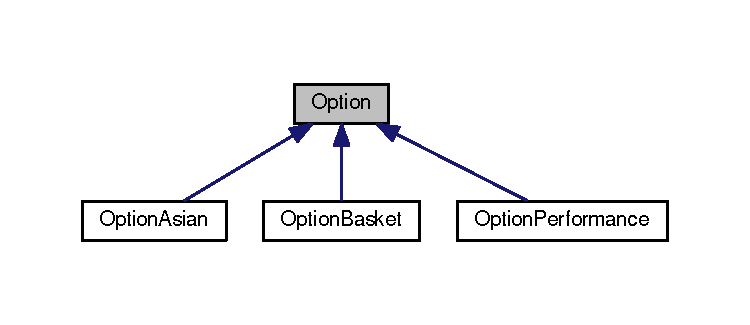
\includegraphics[width=350pt]{classOption__inherit__graph}
\end{center}
\end{figure}
\subsection*{Public Member Functions}
\begin{DoxyCompactItemize}
\item 
\hyperlink{classOption_ad64e6f411a0e0ba09e0179adfb6fc88d}{Option} (double \hyperlink{classOption_a89f0365b68626cc5eb523f12159e0764}{T\-\_\-}, int \hyperlink{classOption_ad424223ea2698144e823c494d625fbe0}{nb\-Time\-Steps\-\_\-}, int \hyperlink{classOption_a65fae5103b50f953f29a86b1a17b4540}{size\-\_\-}, Pnl\-Vect $\ast$\hyperlink{classOption_ae39676c75e7c6592cfcead8abe48b71b}{payoff\-Coeff\-\_\-})
\begin{DoxyCompactList}\small\item\em coefficient permettant le calcul du payoff \end{DoxyCompactList}\item 
virtual \hyperlink{classOption_a04b908a0ba9b1909ae378ca2a07fda61}{$\sim$\-Option} ()
\begin{DoxyCompactList}\small\item\em Destructeur de classe. \end{DoxyCompactList}\item 
virtual double \hyperlink{classOption_abe90882a11f5436077425249e3f32204}{payoff} (const Pnl\-Mat $\ast$path)=0
\begin{DoxyCompactList}\small\item\em Calcule la valeur du payoff sur la trajectoire. \end{DoxyCompactList}\item 
double \hyperlink{classOption_a4307b0dcca6321e0c060abba6a8f4a88}{maturity} ()
\item 
int \hyperlink{classOption_aa170acf6857ed21495c62ab1599f60ae}{nb\-Time\-Steps} ()
\item 
int \hyperlink{classOption_a58d0f66b495003ab29bf0b543ecbe450}{size} ()
\item 
Pnl\-Vect \hyperlink{classOption_aeacd619d109d09331a1fb212b92079ad}{payoff\-Coeff} ()
\item 
double \hyperlink{classOption_a36728dd2492eb49082880d0ef8afe545}{payoff\-Coeff} (int i)
\end{DoxyCompactItemize}
\subsection*{Data Fields}
\begin{DoxyCompactItemize}
\item 
double \hyperlink{classOption_a89f0365b68626cc5eb523f12159e0764}{T\-\_\-}
\item 
int \hyperlink{classOption_ad424223ea2698144e823c494d625fbe0}{nb\-Time\-Steps\-\_\-}
\begin{DoxyCompactList}\small\item\em maturité \end{DoxyCompactList}\item 
int \hyperlink{classOption_a65fae5103b50f953f29a86b1a17b4540}{size\-\_\-}
\begin{DoxyCompactList}\small\item\em nombre de pas de temps de discrétisation \end{DoxyCompactList}\item 
Pnl\-Vect $\ast$ \hyperlink{classOption_ae39676c75e7c6592cfcead8abe48b71b}{payoff\-Coeff\-\_\-}
\begin{DoxyCompactList}\small\item\em dimension du modèle, redondant avec \hyperlink{classBlackScholesModel_ab84e9318c0c1e8a50d5e2f9a70f1256e}{Black\-Scholes\-Model\-::size\-\_\-} \end{DoxyCompactList}\end{DoxyCompactItemize}


\subsection{Detailed Description}
Classe \hyperlink{classOption}{Option} abstraite. 

\subsection{Constructor \& Destructor Documentation}
\hypertarget{classOption_ad64e6f411a0e0ba09e0179adfb6fc88d}{\index{Option@{Option}!Option@{Option}}
\index{Option@{Option}!Option@{Option}}
\subsubsection[{Option}]{\setlength{\rightskip}{0pt plus 5cm}Option\-::\-Option (
\begin{DoxyParamCaption}
\item[{double}]{T\-\_\-, }
\item[{int}]{nb\-Time\-Steps\-\_\-, }
\item[{int}]{size\-\_\-, }
\item[{Pnl\-Vect $\ast$}]{payoff\-Coeff\-\_\-}
\end{DoxyParamCaption}
)}}\label{classOption_ad64e6f411a0e0ba09e0179adfb6fc88d}


coefficient permettant le calcul du payoff 

Constructeur de la classe


\begin{DoxyParams}[1]{Parameters}
\mbox{\tt in}  & {\em maturité} & \\
\hline
\mbox{\tt in}  & {\em nombre} & de pas de temps de discrétisation \\
\hline
\mbox{\tt in}  & {\em dimension} & du modèle, redondant avec \hyperlink{classBlackScholesModel_ab84e9318c0c1e8a50d5e2f9a70f1256e}{Black\-Scholes\-Model\-::size\-\_\-} \\
\hline
\mbox{\tt in}  & {\em coefficient} & permettant le calcul du payoff \\
\hline
\end{DoxyParams}
\hypertarget{classOption_a04b908a0ba9b1909ae378ca2a07fda61}{\index{Option@{Option}!$\sim$\-Option@{$\sim$\-Option}}
\index{$\sim$\-Option@{$\sim$\-Option}!Option@{Option}}
\subsubsection[{$\sim$\-Option}]{\setlength{\rightskip}{0pt plus 5cm}Option\-::$\sim$\-Option (
\begin{DoxyParamCaption}
{}
\end{DoxyParamCaption}
)\hspace{0.3cm}{\ttfamily [virtual]}}}\label{classOption_a04b908a0ba9b1909ae378ca2a07fda61}


Destructeur de classe. 



References payoff\-Coeff\-\_\-.



\subsection{Member Function Documentation}
\hypertarget{classOption_a4307b0dcca6321e0c060abba6a8f4a88}{\index{Option@{Option}!maturity@{maturity}}
\index{maturity@{maturity}!Option@{Option}}
\subsubsection[{maturity}]{\setlength{\rightskip}{0pt plus 5cm}double Option\-::maturity (
\begin{DoxyParamCaption}
{}
\end{DoxyParamCaption}
)}}\label{classOption_a4307b0dcca6321e0c060abba6a8f4a88}


References T\-\_\-.

\hypertarget{classOption_aa170acf6857ed21495c62ab1599f60ae}{\index{Option@{Option}!nb\-Time\-Steps@{nb\-Time\-Steps}}
\index{nb\-Time\-Steps@{nb\-Time\-Steps}!Option@{Option}}
\subsubsection[{nb\-Time\-Steps}]{\setlength{\rightskip}{0pt plus 5cm}int Option\-::nb\-Time\-Steps (
\begin{DoxyParamCaption}
{}
\end{DoxyParamCaption}
)}}\label{classOption_aa170acf6857ed21495c62ab1599f60ae}


References nb\-Time\-Steps\-\_\-.

\hypertarget{classOption_abe90882a11f5436077425249e3f32204}{\index{Option@{Option}!payoff@{payoff}}
\index{payoff@{payoff}!Option@{Option}}
\subsubsection[{payoff}]{\setlength{\rightskip}{0pt plus 5cm}virtual double Option\-::payoff (
\begin{DoxyParamCaption}
\item[{const Pnl\-Mat $\ast$}]{path}
\end{DoxyParamCaption}
)\hspace{0.3cm}{\ttfamily [pure virtual]}}}\label{classOption_abe90882a11f5436077425249e3f32204}


Calcule la valeur du payoff sur la trajectoire. 


\begin{DoxyParams}[1]{Parameters}
\mbox{\tt in}  & {\em path} & est une matrice de taille (N+1) x d contenant une trajectoire du modèle telle que créée par la fonction asset. \\
\hline
\end{DoxyParams}
\begin{DoxyReturn}{Returns}
phi(trajectoire) 
\end{DoxyReturn}


Implemented in \hyperlink{classOptionAsian_a4b7fefbd591f8a77e43078e1245801ea}{Option\-Asian}, \hyperlink{classOptionBasket_ab513ea6e21f7803ef5e71227170faa16}{Option\-Basket}, and \hyperlink{classOptionPerformance_a567dcb592f5e20203f590118d9542d94}{Option\-Performance}.



Referenced by Monte\-Carlo\-::delta(), Monte\-Carlo\-::hedging\-P\-And\-L(), and Monte\-Carlo\-::price().

\hypertarget{classOption_aeacd619d109d09331a1fb212b92079ad}{\index{Option@{Option}!payoff\-Coeff@{payoff\-Coeff}}
\index{payoff\-Coeff@{payoff\-Coeff}!Option@{Option}}
\subsubsection[{payoff\-Coeff}]{\setlength{\rightskip}{0pt plus 5cm}Pnl\-Vect Option\-::payoff\-Coeff (
\begin{DoxyParamCaption}
{}
\end{DoxyParamCaption}
)}}\label{classOption_aeacd619d109d09331a1fb212b92079ad}


References payoff\-Coeff\-\_\-.

\hypertarget{classOption_a36728dd2492eb49082880d0ef8afe545}{\index{Option@{Option}!payoff\-Coeff@{payoff\-Coeff}}
\index{payoff\-Coeff@{payoff\-Coeff}!Option@{Option}}
\subsubsection[{payoff\-Coeff}]{\setlength{\rightskip}{0pt plus 5cm}double Option\-::payoff\-Coeff (
\begin{DoxyParamCaption}
\item[{int}]{i}
\end{DoxyParamCaption}
)}}\label{classOption_a36728dd2492eb49082880d0ef8afe545}


References payoff\-Coeff\-\_\-.

\hypertarget{classOption_a58d0f66b495003ab29bf0b543ecbe450}{\index{Option@{Option}!size@{size}}
\index{size@{size}!Option@{Option}}
\subsubsection[{size}]{\setlength{\rightskip}{0pt plus 5cm}int Option\-::size (
\begin{DoxyParamCaption}
{}
\end{DoxyParamCaption}
)}}\label{classOption_a58d0f66b495003ab29bf0b543ecbe450}


References size\-\_\-.



\subsection{Field Documentation}
\hypertarget{classOption_ad424223ea2698144e823c494d625fbe0}{\index{Option@{Option}!nb\-Time\-Steps\-\_\-@{nb\-Time\-Steps\-\_\-}}
\index{nb\-Time\-Steps\-\_\-@{nb\-Time\-Steps\-\_\-}!Option@{Option}}
\subsubsection[{nb\-Time\-Steps\-\_\-}]{\setlength{\rightskip}{0pt plus 5cm}int Option\-::nb\-Time\-Steps\-\_\-}}\label{classOption_ad424223ea2698144e823c494d625fbe0}


maturité 



Referenced by Monte\-Carlo\-::delta(), Monte\-Carlo\-::hedging\-P\-And\-L(), Monte\-Carlo\-::\-Monte\-Carlo(), nb\-Time\-Steps(), Option\-Asian\-::payoff(), Option\-Performance\-::payoff(), Option\-Basket\-::payoff(), and Monte\-Carlo\-::price().

\hypertarget{classOption_ae39676c75e7c6592cfcead8abe48b71b}{\index{Option@{Option}!payoff\-Coeff\-\_\-@{payoff\-Coeff\-\_\-}}
\index{payoff\-Coeff\-\_\-@{payoff\-Coeff\-\_\-}!Option@{Option}}
\subsubsection[{payoff\-Coeff\-\_\-}]{\setlength{\rightskip}{0pt plus 5cm}Pnl\-Vect$\ast$ Option\-::payoff\-Coeff\-\_\-}}\label{classOption_ae39676c75e7c6592cfcead8abe48b71b}


dimension du modèle, redondant avec \hyperlink{classBlackScholesModel_ab84e9318c0c1e8a50d5e2f9a70f1256e}{Black\-Scholes\-Model\-::size\-\_\-} 



Referenced by Option\-Asian\-::payoff(), Option\-Performance\-::payoff(), Option\-Basket\-::payoff(), payoff\-Coeff(), and $\sim$\-Option().

\hypertarget{classOption_a65fae5103b50f953f29a86b1a17b4540}{\index{Option@{Option}!size\-\_\-@{size\-\_\-}}
\index{size\-\_\-@{size\-\_\-}!Option@{Option}}
\subsubsection[{size\-\_\-}]{\setlength{\rightskip}{0pt plus 5cm}int Option\-::size\-\_\-}}\label{classOption_a65fae5103b50f953f29a86b1a17b4540}


nombre de pas de temps de discrétisation 



Referenced by Option\-Asian\-::payoff(), Option\-Performance\-::payoff(), Option\-Basket\-::payoff(), and size().

\hypertarget{classOption_a89f0365b68626cc5eb523f12159e0764}{\index{Option@{Option}!T\-\_\-@{T\-\_\-}}
\index{T\-\_\-@{T\-\_\-}!Option@{Option}}
\subsubsection[{T\-\_\-}]{\setlength{\rightskip}{0pt plus 5cm}double Option\-::\-T\-\_\-}}\label{classOption_a89f0365b68626cc5eb523f12159e0764}


Referenced by Monte\-Carlo\-::delta(), Monte\-Carlo\-::hedging\-P\-And\-L(), maturity(), and Monte\-Carlo\-::price().



The documentation for this class was generated from the following files\-:\begin{DoxyCompactItemize}
\item 
/user/0/.\-base/charmont/home/\-Documents/3\-A/\-Projet/pricer\-Monte\-Carlo/src/\hyperlink{Option_8hpp}{Option.\-hpp}\item 
/user/0/.\-base/charmont/home/\-Documents/3\-A/\-Projet/pricer\-Monte\-Carlo/src/\hyperlink{Option_8cpp}{Option.\-cpp}\end{DoxyCompactItemize}

\hypertarget{classOptionAsian}{\section{Option\-Asian Class Reference}
\label{classOptionAsian}\index{Option\-Asian@{Option\-Asian}}
}


{\ttfamily \#include $<$Option\-Asian.\-hpp$>$}



Inheritance diagram for Option\-Asian\-:\nopagebreak
\begin{figure}[H]
\begin{center}
\leavevmode
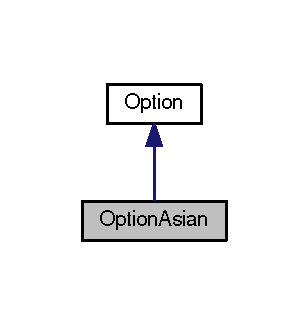
\includegraphics[width=148pt]{classOptionAsian__inherit__graph}
\end{center}
\end{figure}


Collaboration diagram for Option\-Asian\-:\nopagebreak
\begin{figure}[H]
\begin{center}
\leavevmode
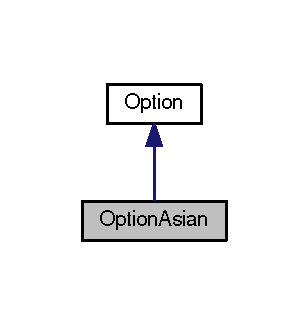
\includegraphics[width=148pt]{classOptionAsian__coll__graph}
\end{center}
\end{figure}
\subsection*{Public Member Functions}
\begin{DoxyCompactItemize}
\item 
\hyperlink{classOptionAsian_aa2ebea7bae19cfae1df2488459834624}{Option\-Asian} (double \hyperlink{classOption_a89f0365b68626cc5eb523f12159e0764}{T\-\_\-}, int \hyperlink{classOption_ad424223ea2698144e823c494d625fbe0}{nb\-Time\-Steps\-\_\-}, int \hyperlink{classOption_a65fae5103b50f953f29a86b1a17b4540}{size\-\_\-}, Pnl\-Vect $\ast$\hyperlink{classOption_ae39676c75e7c6592cfcead8abe48b71b}{payoff\-Coeff\-\_\-}, double \hyperlink{classOptionAsian_a2b1952985f78ae8fd471275556fec724}{strike\-\_\-})
\item 
virtual double \hyperlink{classOptionAsian_a4b7fefbd591f8a77e43078e1245801ea}{payoff} (const Pnl\-Mat $\ast$path)
\begin{DoxyCompactList}\small\item\em Calcule la valeur du payoff sur la trajectoire. \end{DoxyCompactList}\item 
double \hyperlink{classOptionAsian_a067e53c46d0746b3961609a5a1422f2b}{strike} ()
\end{DoxyCompactItemize}
\subsection*{Protected Attributes}
\begin{DoxyCompactItemize}
\item 
double \hyperlink{classOptionAsian_a2b1952985f78ae8fd471275556fec724}{strike\-\_\-}
\end{DoxyCompactItemize}
\subsection*{Additional Inherited Members}


\subsection{Constructor \& Destructor Documentation}
\hypertarget{classOptionAsian_aa2ebea7bae19cfae1df2488459834624}{\index{Option\-Asian@{Option\-Asian}!Option\-Asian@{Option\-Asian}}
\index{Option\-Asian@{Option\-Asian}!OptionAsian@{Option\-Asian}}
\subsubsection[{Option\-Asian}]{\setlength{\rightskip}{0pt plus 5cm}Option\-Asian\-::\-Option\-Asian (
\begin{DoxyParamCaption}
\item[{double}]{T\-\_\-, }
\item[{int}]{nb\-Time\-Steps\-\_\-, }
\item[{int}]{size\-\_\-, }
\item[{Pnl\-Vect $\ast$}]{payoff\-Coeff\-\_\-, }
\item[{double}]{strike\-\_\-}
\end{DoxyParamCaption}
)}}\label{classOptionAsian_aa2ebea7bae19cfae1df2488459834624}


\subsection{Member Function Documentation}
\hypertarget{classOptionAsian_a4b7fefbd591f8a77e43078e1245801ea}{\index{Option\-Asian@{Option\-Asian}!payoff@{payoff}}
\index{payoff@{payoff}!OptionAsian@{Option\-Asian}}
\subsubsection[{payoff}]{\setlength{\rightskip}{0pt plus 5cm}double Option\-Asian\-::payoff (
\begin{DoxyParamCaption}
\item[{const Pnl\-Mat $\ast$}]{path}
\end{DoxyParamCaption}
)\hspace{0.3cm}{\ttfamily [virtual]}}}\label{classOptionAsian_a4b7fefbd591f8a77e43078e1245801ea}


Calcule la valeur du payoff sur la trajectoire. 


\begin{DoxyParams}[1]{Parameters}
\mbox{\tt in}  & {\em path} & est une matrice de taille (N+1) x d contenant une trajectoire du modèle telle que créée par la fonction asset. \\
\hline
\end{DoxyParams}
\begin{DoxyReturn}{Returns}
phi(trajectoire) 
\end{DoxyReturn}


Implements \hyperlink{classOption_abe90882a11f5436077425249e3f32204}{Option}.



References Option\-::nb\-Time\-Steps\-\_\-, Option\-::payoff\-Coeff\-\_\-, Option\-::size\-\_\-, and strike\-\_\-.

\hypertarget{classOptionAsian_a067e53c46d0746b3961609a5a1422f2b}{\index{Option\-Asian@{Option\-Asian}!strike@{strike}}
\index{strike@{strike}!OptionAsian@{Option\-Asian}}
\subsubsection[{strike}]{\setlength{\rightskip}{0pt plus 5cm}double Option\-Asian\-::strike (
\begin{DoxyParamCaption}
{}
\end{DoxyParamCaption}
)}}\label{classOptionAsian_a067e53c46d0746b3961609a5a1422f2b}


References strike\-\_\-.



\subsection{Field Documentation}
\hypertarget{classOptionAsian_a2b1952985f78ae8fd471275556fec724}{\index{Option\-Asian@{Option\-Asian}!strike\-\_\-@{strike\-\_\-}}
\index{strike\-\_\-@{strike\-\_\-}!OptionAsian@{Option\-Asian}}
\subsubsection[{strike\-\_\-}]{\setlength{\rightskip}{0pt plus 5cm}double Option\-Asian\-::strike\-\_\-\hspace{0.3cm}{\ttfamily [protected]}}}\label{classOptionAsian_a2b1952985f78ae8fd471275556fec724}


Referenced by payoff(), and strike().



The documentation for this class was generated from the following files\-:\begin{DoxyCompactItemize}
\item 
/user/0/.\-base/charmont/home/\-Documents/3\-A/\-Projet/pricer\-Monte\-Carlo/src/\hyperlink{OptionAsian_8hpp}{Option\-Asian.\-hpp}\item 
/user/0/.\-base/charmont/home/\-Documents/3\-A/\-Projet/pricer\-Monte\-Carlo/src/\hyperlink{OptionAsian_8cpp}{Option\-Asian.\-cpp}\end{DoxyCompactItemize}

\hypertarget{classOptionBasket}{\section{Option\-Basket Class Reference}
\label{classOptionBasket}\index{Option\-Basket@{Option\-Basket}}
}


{\ttfamily \#include $<$Option\-Basket.\-hpp$>$}



Inheritance diagram for Option\-Basket\-:\nopagebreak
\begin{figure}[H]
\begin{center}
\leavevmode
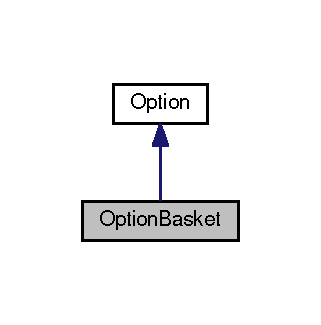
\includegraphics[width=154pt]{classOptionBasket__inherit__graph}
\end{center}
\end{figure}


Collaboration diagram for Option\-Basket\-:\nopagebreak
\begin{figure}[H]
\begin{center}
\leavevmode
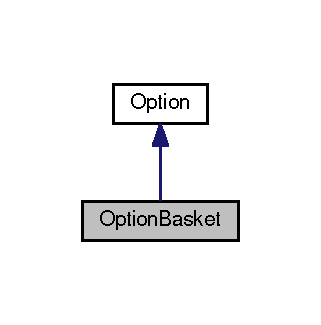
\includegraphics[width=154pt]{classOptionBasket__coll__graph}
\end{center}
\end{figure}
\subsection*{Public Member Functions}
\begin{DoxyCompactItemize}
\item 
\hyperlink{classOptionBasket_ab04ed860918646e5e7e4410a2aca7e60}{Option\-Basket} (double \hyperlink{classOption_a89f0365b68626cc5eb523f12159e0764}{T\-\_\-}, int \hyperlink{classOption_ad424223ea2698144e823c494d625fbe0}{nb\-Time\-Steps\-\_\-}, int \hyperlink{classOption_a65fae5103b50f953f29a86b1a17b4540}{size\-\_\-}, Pnl\-Vect $\ast$\hyperlink{classOption_ae39676c75e7c6592cfcead8abe48b71b}{payoff\-Coeff\-\_\-}, double \hyperlink{classOptionBasket_a577ab909d0049dd2036b6751f64f93f4}{strike\-\_\-})
\item 
virtual double \hyperlink{classOptionBasket_ab513ea6e21f7803ef5e71227170faa16}{payoff} (const Pnl\-Mat $\ast$path)
\begin{DoxyCompactList}\small\item\em Calcule la valeur du payoff sur la trajectoire. \end{DoxyCompactList}\item 
double \hyperlink{classOptionBasket_a134cca36a78858747302d7b76623ea1b}{strike} ()
\end{DoxyCompactItemize}
\subsection*{Protected Attributes}
\begin{DoxyCompactItemize}
\item 
double \hyperlink{classOptionBasket_a577ab909d0049dd2036b6751f64f93f4}{strike\-\_\-}
\end{DoxyCompactItemize}
\subsection*{Additional Inherited Members}


\subsection{Constructor \& Destructor Documentation}
\hypertarget{classOptionBasket_ab04ed860918646e5e7e4410a2aca7e60}{\index{Option\-Basket@{Option\-Basket}!Option\-Basket@{Option\-Basket}}
\index{Option\-Basket@{Option\-Basket}!OptionBasket@{Option\-Basket}}
\subsubsection[{Option\-Basket}]{\setlength{\rightskip}{0pt plus 5cm}Option\-Basket\-::\-Option\-Basket (
\begin{DoxyParamCaption}
\item[{double}]{T\-\_\-, }
\item[{int}]{nb\-Time\-Steps\-\_\-, }
\item[{int}]{size\-\_\-, }
\item[{Pnl\-Vect $\ast$}]{payoff\-Coeff\-\_\-, }
\item[{double}]{strike\-\_\-}
\end{DoxyParamCaption}
)}}\label{classOptionBasket_ab04ed860918646e5e7e4410a2aca7e60}


\subsection{Member Function Documentation}
\hypertarget{classOptionBasket_ab513ea6e21f7803ef5e71227170faa16}{\index{Option\-Basket@{Option\-Basket}!payoff@{payoff}}
\index{payoff@{payoff}!OptionBasket@{Option\-Basket}}
\subsubsection[{payoff}]{\setlength{\rightskip}{0pt plus 5cm}double Option\-Basket\-::payoff (
\begin{DoxyParamCaption}
\item[{const Pnl\-Mat $\ast$}]{path}
\end{DoxyParamCaption}
)\hspace{0.3cm}{\ttfamily [virtual]}}}\label{classOptionBasket_ab513ea6e21f7803ef5e71227170faa16}


Calcule la valeur du payoff sur la trajectoire. 


\begin{DoxyParams}[1]{Parameters}
\mbox{\tt in}  & {\em path} & est une matrice de taille (N+1) x d contenant une trajectoire du modèle telle que créée par la fonction asset. \\
\hline
\end{DoxyParams}
\begin{DoxyReturn}{Returns}
phi(trajectoire) 
\end{DoxyReturn}


Implements \hyperlink{classOption_abe90882a11f5436077425249e3f32204}{Option}.



References Option\-::nb\-Time\-Steps\-\_\-, Option\-::payoff\-Coeff\-\_\-, Option\-::size\-\_\-, and strike\-\_\-.

\hypertarget{classOptionBasket_a134cca36a78858747302d7b76623ea1b}{\index{Option\-Basket@{Option\-Basket}!strike@{strike}}
\index{strike@{strike}!OptionBasket@{Option\-Basket}}
\subsubsection[{strike}]{\setlength{\rightskip}{0pt plus 5cm}double Option\-Basket\-::strike (
\begin{DoxyParamCaption}
{}
\end{DoxyParamCaption}
)}}\label{classOptionBasket_a134cca36a78858747302d7b76623ea1b}


References strike\-\_\-.



\subsection{Field Documentation}
\hypertarget{classOptionBasket_a577ab909d0049dd2036b6751f64f93f4}{\index{Option\-Basket@{Option\-Basket}!strike\-\_\-@{strike\-\_\-}}
\index{strike\-\_\-@{strike\-\_\-}!OptionBasket@{Option\-Basket}}
\subsubsection[{strike\-\_\-}]{\setlength{\rightskip}{0pt plus 5cm}double Option\-Basket\-::strike\-\_\-\hspace{0.3cm}{\ttfamily [protected]}}}\label{classOptionBasket_a577ab909d0049dd2036b6751f64f93f4}


Referenced by payoff(), and strike().



The documentation for this class was generated from the following files\-:\begin{DoxyCompactItemize}
\item 
/user/0/.\-base/charmont/home/\-Documents/3\-A/\-Projet/pricer\-Monte\-Carlo/src/\hyperlink{OptionBasket_8hpp}{Option\-Basket.\-hpp}\item 
/user/0/.\-base/charmont/home/\-Documents/3\-A/\-Projet/pricer\-Monte\-Carlo/src/\hyperlink{OptionBasket_8cpp}{Option\-Basket.\-cpp}\end{DoxyCompactItemize}

\hypertarget{classOptionPerformance}{\section{Option\-Performance Class Reference}
\label{classOptionPerformance}\index{Option\-Performance@{Option\-Performance}}
}


{\ttfamily \#include $<$Option\-Performance.\-hpp$>$}



Inheritance diagram for Option\-Performance\-:
\nopagebreak
\begin{figure}[H]
\begin{center}
\leavevmode
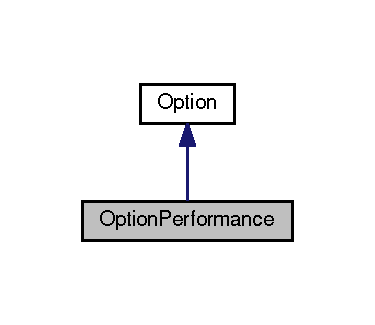
\includegraphics[width=180pt]{classOptionPerformance__inherit__graph}
\end{center}
\end{figure}


Collaboration diagram for Option\-Performance\-:
\nopagebreak
\begin{figure}[H]
\begin{center}
\leavevmode
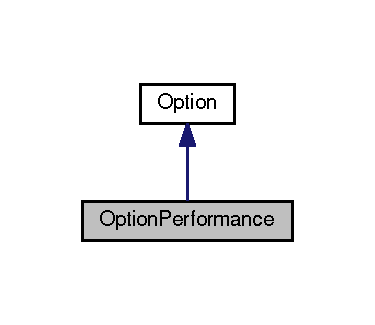
\includegraphics[width=180pt]{classOptionPerformance__coll__graph}
\end{center}
\end{figure}
\subsection*{Public Member Functions}
\begin{DoxyCompactItemize}
\item 
\hyperlink{classOptionPerformance_a7d4af76675e997e1b3f49289167c5a67}{Option\-Performance} (double \hyperlink{classOption_a89f0365b68626cc5eb523f12159e0764}{T\-\_\-}, int \hyperlink{classOption_ad424223ea2698144e823c494d625fbe0}{nb\-Time\-Steps\-\_\-}, int \hyperlink{classOption_a65fae5103b50f953f29a86b1a17b4540}{size\-\_\-}, Pnl\-Vect $\ast$\hyperlink{classOption_ae39676c75e7c6592cfcead8abe48b71b}{payoff\-Coeff\-\_\-})
\item 
virtual double \hyperlink{classOptionPerformance_a567dcb592f5e20203f590118d9542d94}{payoff} (const Pnl\-Mat $\ast$path)
\begin{DoxyCompactList}\small\item\em Calcule la valeur du payoff sur la trajectoire. \end{DoxyCompactList}\end{DoxyCompactItemize}
\subsection*{Additional Inherited Members}


\subsection{Constructor \& Destructor Documentation}
\hypertarget{classOptionPerformance_a7d4af76675e997e1b3f49289167c5a67}{\index{Option\-Performance@{Option\-Performance}!Option\-Performance@{Option\-Performance}}
\index{Option\-Performance@{Option\-Performance}!OptionPerformance@{Option\-Performance}}
\subsubsection[{Option\-Performance}]{\setlength{\rightskip}{0pt plus 5cm}Option\-Performance\-::\-Option\-Performance (
\begin{DoxyParamCaption}
\item[{double}]{T\-\_\-, }
\item[{int}]{nb\-Time\-Steps\-\_\-, }
\item[{int}]{size\-\_\-, }
\item[{Pnl\-Vect $\ast$}]{payoff\-Coeff\-\_\-}
\end{DoxyParamCaption}
)}}\label{classOptionPerformance_a7d4af76675e997e1b3f49289167c5a67}


\subsection{Member Function Documentation}
\hypertarget{classOptionPerformance_a567dcb592f5e20203f590118d9542d94}{\index{Option\-Performance@{Option\-Performance}!payoff@{payoff}}
\index{payoff@{payoff}!OptionPerformance@{Option\-Performance}}
\subsubsection[{payoff}]{\setlength{\rightskip}{0pt plus 5cm}double Option\-Performance\-::payoff (
\begin{DoxyParamCaption}
\item[{const Pnl\-Mat $\ast$}]{path}
\end{DoxyParamCaption}
)\hspace{0.3cm}{\ttfamily [virtual]}}}\label{classOptionPerformance_a567dcb592f5e20203f590118d9542d94}


Calcule la valeur du payoff sur la trajectoire. 


\begin{DoxyParams}[1]{Parameters}
\mbox{\tt in}  & {\em path} & est une matrice de taille (N+1) x d contenant une trajectoire du modèle telle que créée par la fonction asset. \\
\hline
\end{DoxyParams}
\begin{DoxyReturn}{Returns}
phi(trajectoire) 
\end{DoxyReturn}


Implements \hyperlink{classOption_abe90882a11f5436077425249e3f32204}{Option}.



References Option\-::nb\-Time\-Steps\-\_\-, Option\-::payoff\-Coeff\-\_\-, and Option\-::size\-\_\-.



The documentation for this class was generated from the following files\-:\begin{DoxyCompactItemize}
\item 
/user/2/.\-base/margueed/home/pricer\-Monte\-Carlo/src/\hyperlink{OptionPerformance_8hpp}{Option\-Performance.\-hpp}\item 
/user/2/.\-base/margueed/home/pricer\-Monte\-Carlo/src/\hyperlink{OptionPerformance_8cpp}{Option\-Performance.\-cpp}\end{DoxyCompactItemize}

\hypertarget{classParam}{\section{Param Class Reference}
\label{classParam}\index{Param@{Param}}
}


{\ttfamily \#include $<$parser.\-hpp$>$}



Inheritance diagram for Param\-:
\nopagebreak
\begin{figure}[H]
\begin{center}
\leavevmode
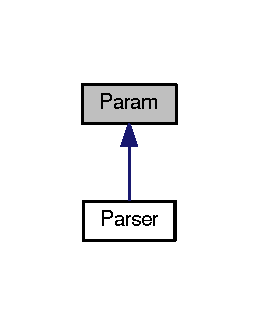
\includegraphics[width=124pt]{classParam__inherit__graph}
\end{center}
\end{figure}
\subsection*{Public Member Functions}
\begin{DoxyCompactItemize}
\item 
\hyperlink{classParam_ae0eeef2ab32df12ccc4e9d2174d6e91a}{Param} ()
\item 
\hyperlink{classParam_a37fea09e1a1e9b563d9a99ae07651cfc}{Param} (const \hyperlink{classParam}{Param} \&)
\item 
\hyperlink{classParam_a63814ed15af3910f8899dbd6853a7e05}{$\sim$\-Param} ()
\item 
\hyperlink{classParam}{Param} \& \hyperlink{classParam_a4379b839d0232f2be88cb0f0ea22e764}{operator=} (const \hyperlink{classParam}{Param} \&P)
\item 
{\footnotesize template$<$typename T $>$ }\\bool \hyperlink{classParam_ac6c8cda9e2a70f76b6fb68434ade63a7}{extract} (const std\-::string \&key, T \&out, bool go\-\_\-on=true) const 
\item 
bool \hyperlink{classParam_a4747df3d3a71c4ba0903021f53852a51}{extract} (const std\-::string \&key, Pnl\-Vect $\ast$\&out, int size, bool go\-\_\-on=true) const 
\begin{DoxyCompactList}\small\item\em Set out according to P. \end{DoxyCompactList}\item 
{\footnotesize template$<$typename T $>$ }\\bool \hyperlink{classParam_a6e7845fcfd27605274ea017b27122344}{set} (const std\-::string \&key, const T \&in)
\item 
{\footnotesize template$<$typename T $>$ }\\void \hyperlink{classParam_a2d37d55e8112a67ac0fdbd719b141837}{insert} (const std\-::string \&key, const \hyperlink{parser_8hpp_a90856b8fb3f1a65845ffec1ec2884c0f}{T\-\_\-type} \&t, const T \&in)
\begin{DoxyCompactList}\small\item\em Insert a new pair in the map or set M\mbox{[}key\mbox{]} to the new value if the key already exists in the map. \end{DoxyCompactList}\item 
void \hyperlink{classParam_a05fdfe029c450d1607e64cda216ed7ac}{print} () const 
\end{DoxyCompactItemize}
\subsection*{Data Fields}
\begin{DoxyCompactItemize}
\item 
\hyperlink{parser_8hpp_a77c3bfcf208503ef5164669afcd00ffe}{Hash} \hyperlink{classParam_ab671c1688f5247604d23ed990c90fd36}{M}
\end{DoxyCompactItemize}
\subsection*{Private Member Functions}
\begin{DoxyCompactItemize}
\item 
bool \hyperlink{classParam_aa33a739416b3ac5b16621b047a6af606}{check\-\_\-if\-\_\-key} (Hash\-::const\-\_\-iterator \&it, const std\-::string \&key) const 
\item 
{\footnotesize template$<$class Archive $>$ }\\void \hyperlink{classParam_a85bdbba6027dbd3e8001ab3eb8408814}{serialize} (Archive \&ar, const unsigned int version)
\end{DoxyCompactItemize}
\subsection*{Friends}
\begin{DoxyCompactItemize}
\item 
class \hyperlink{classParam_ac98d07dd8f7b70e16ccb9a01abf56b9c}{boost\-::serialization\-::access}
\end{DoxyCompactItemize}


\subsection{Constructor \& Destructor Documentation}
\hypertarget{classParam_ae0eeef2ab32df12ccc4e9d2174d6e91a}{\index{Param@{Param}!Param@{Param}}
\index{Param@{Param}!Param@{Param}}
\subsubsection[{Param}]{\setlength{\rightskip}{0pt plus 5cm}Param\-::\-Param (
\begin{DoxyParamCaption}
{}
\end{DoxyParamCaption}
)\hspace{0.3cm}{\ttfamily [inline]}}}\label{classParam_ae0eeef2ab32df12ccc4e9d2174d6e91a}
\hypertarget{classParam_a37fea09e1a1e9b563d9a99ae07651cfc}{\index{Param@{Param}!Param@{Param}}
\index{Param@{Param}!Param@{Param}}
\subsubsection[{Param}]{\setlength{\rightskip}{0pt plus 5cm}Param\-::\-Param (
\begin{DoxyParamCaption}
\item[{const {\bf Param} \&}]{P}
\end{DoxyParamCaption}
)}}\label{classParam_a37fea09e1a1e9b563d9a99ae07651cfc}


References M.

\hypertarget{classParam_a63814ed15af3910f8899dbd6853a7e05}{\index{Param@{Param}!$\sim$\-Param@{$\sim$\-Param}}
\index{$\sim$\-Param@{$\sim$\-Param}!Param@{Param}}
\subsubsection[{$\sim$\-Param}]{\setlength{\rightskip}{0pt plus 5cm}Param\-::$\sim$\-Param (
\begin{DoxyParamCaption}
{}
\end{DoxyParamCaption}
)}}\label{classParam_a63814ed15af3910f8899dbd6853a7e05}


References M.



\subsection{Member Function Documentation}
\hypertarget{classParam_aa33a739416b3ac5b16621b047a6af606}{\index{Param@{Param}!check\-\_\-if\-\_\-key@{check\-\_\-if\-\_\-key}}
\index{check\-\_\-if\-\_\-key@{check\-\_\-if\-\_\-key}!Param@{Param}}
\subsubsection[{check\-\_\-if\-\_\-key}]{\setlength{\rightskip}{0pt plus 5cm}bool Param\-::check\-\_\-if\-\_\-key (
\begin{DoxyParamCaption}
\item[{Hash\-::const\-\_\-iterator \&}]{it, }
\item[{const std\-::string \&}]{key}
\end{DoxyParamCaption}
) const\hspace{0.3cm}{\ttfamily [private]}}}\label{classParam_aa33a739416b3ac5b16621b047a6af606}


References M.



Referenced by extract().

\hypertarget{classParam_ac6c8cda9e2a70f76b6fb68434ade63a7}{\index{Param@{Param}!extract@{extract}}
\index{extract@{extract}!Param@{Param}}
\subsubsection[{extract}]{\setlength{\rightskip}{0pt plus 5cm}template$<$typename T $>$ bool Param\-::extract (
\begin{DoxyParamCaption}
\item[{const std\-::string \&}]{key, }
\item[{T \&}]{out, }
\item[{bool}]{go\-\_\-on = {\ttfamily true}}
\end{DoxyParamCaption}
) const\hspace{0.3cm}{\ttfamily [inline]}}}\label{classParam_ac6c8cda9e2a70f76b6fb68434ade63a7}


References check\-\_\-if\-\_\-key().



Referenced by main().

\hypertarget{classParam_a4747df3d3a71c4ba0903021f53852a51}{\index{Param@{Param}!extract@{extract}}
\index{extract@{extract}!Param@{Param}}
\subsubsection[{extract}]{\setlength{\rightskip}{0pt plus 5cm}bool Param\-::extract (
\begin{DoxyParamCaption}
\item[{const std\-::string \&}]{key, }
\item[{Pnl\-Vect $\ast$\&}]{out, }
\item[{int}]{size, }
\item[{bool}]{go\-\_\-on = {\ttfamily true}}
\end{DoxyParamCaption}
) const}}\label{classParam_a4747df3d3a71c4ba0903021f53852a51}


Set out according to P. 


\begin{DoxyParams}{Parameters}
{\em key} & the key to be looked for in the map \\
\hline
{\em out} & (output) set to the value associated to key in the map \\
\hline
{\em size} & size of the vector to be stored \\
\hline
{\em go\-\_\-on} & a boolean, if false and key is not found in the map, the abort function is called \\
\hline
\end{DoxyParams}


References check\-\_\-if\-\_\-key().

\hypertarget{classParam_a2d37d55e8112a67ac0fdbd719b141837}{\index{Param@{Param}!insert@{insert}}
\index{insert@{insert}!Param@{Param}}
\subsubsection[{insert}]{\setlength{\rightskip}{0pt plus 5cm}template$<$typename T $>$ void Param\-::insert (
\begin{DoxyParamCaption}
\item[{const std\-::string \&}]{key, }
\item[{const {\bf T\-\_\-type} \&}]{t, }
\item[{const T \&}]{in}
\end{DoxyParamCaption}
)\hspace{0.3cm}{\ttfamily [inline]}}}\label{classParam_a2d37d55e8112a67ac0fdbd719b141837}


Insert a new pair in the map or set M\mbox{[}key\mbox{]} to the new value if the key already exists in the map. 


\begin{DoxyTemplParams}{Template Parameters}
{\em T} & the template type of the element to be inserted \\
\hline
\end{DoxyTemplParams}

\begin{DoxyParams}{Parameters}
{\em key} & the key \\
\hline
{\em t} & the type of the elements as an integer \\
\hline
{\em in} & the element itself \\
\hline
\end{DoxyParams}


References M, Type\-Val\-::type, and Type\-Val\-::\-Val.

\hypertarget{classParam_a4379b839d0232f2be88cb0f0ea22e764}{\index{Param@{Param}!operator=@{operator=}}
\index{operator=@{operator=}!Param@{Param}}
\subsubsection[{operator=}]{\setlength{\rightskip}{0pt plus 5cm}{\bf Param} \& Param\-::operator= (
\begin{DoxyParamCaption}
\item[{const {\bf Param} \&}]{P}
\end{DoxyParamCaption}
)}}\label{classParam_a4379b839d0232f2be88cb0f0ea22e764}


References M.

\hypertarget{classParam_a05fdfe029c450d1607e64cda216ed7ac}{\index{Param@{Param}!print@{print}}
\index{print@{print}!Param@{Param}}
\subsubsection[{print}]{\setlength{\rightskip}{0pt plus 5cm}void Param\-::print (
\begin{DoxyParamCaption}
{}
\end{DoxyParamCaption}
) const\hspace{0.3cm}{\ttfamily [inline]}}}\label{classParam_a05fdfe029c450d1607e64cda216ed7ac}


References M.

\hypertarget{classParam_a85bdbba6027dbd3e8001ab3eb8408814}{\index{Param@{Param}!serialize@{serialize}}
\index{serialize@{serialize}!Param@{Param}}
\subsubsection[{serialize}]{\setlength{\rightskip}{0pt plus 5cm}template$<$class Archive $>$ void Param\-::serialize (
\begin{DoxyParamCaption}
\item[{Archive \&}]{ar, }
\item[{const unsigned int}]{version}
\end{DoxyParamCaption}
)\hspace{0.3cm}{\ttfamily [inline]}, {\ttfamily [private]}}}\label{classParam_a85bdbba6027dbd3e8001ab3eb8408814}


References M.

\hypertarget{classParam_a6e7845fcfd27605274ea017b27122344}{\index{Param@{Param}!set@{set}}
\index{set@{set}!Param@{Param}}
\subsubsection[{set}]{\setlength{\rightskip}{0pt plus 5cm}template$<$typename T $>$ bool Param\-::set (
\begin{DoxyParamCaption}
\item[{const std\-::string \&}]{key, }
\item[{const T \&}]{in}
\end{DoxyParamCaption}
)\hspace{0.3cm}{\ttfamily [inline]}}}\label{classParam_a6e7845fcfd27605274ea017b27122344}


References M.



\subsection{Friends And Related Function Documentation}
\hypertarget{classParam_ac98d07dd8f7b70e16ccb9a01abf56b9c}{\index{Param@{Param}!boost\-::serialization\-::access@{boost\-::serialization\-::access}}
\index{boost\-::serialization\-::access@{boost\-::serialization\-::access}!Param@{Param}}
\subsubsection[{boost\-::serialization\-::access}]{\setlength{\rightskip}{0pt plus 5cm}friend class boost\-::serialization\-::access\hspace{0.3cm}{\ttfamily [friend]}}}\label{classParam_ac98d07dd8f7b70e16ccb9a01abf56b9c}


\subsection{Field Documentation}
\hypertarget{classParam_ab671c1688f5247604d23ed990c90fd36}{\index{Param@{Param}!M@{M}}
\index{M@{M}!Param@{Param}}
\subsubsection[{M}]{\setlength{\rightskip}{0pt plus 5cm}{\bf Hash} Param\-::\-M}}\label{classParam_ab671c1688f5247604d23ed990c90fd36}


Referenced by Parser\-::add(), check\-\_\-if\-\_\-key(), insert(), operator=(), Param(), print(), serialize(), set(), and $\sim$\-Param().



The documentation for this class was generated from the following files\-:\begin{DoxyCompactItemize}
\item 
/user/2/.\-base/margueed/home/pricer\-Monte\-Carlo/src/\hyperlink{parser_8hpp}{parser.\-hpp}\item 
/user/2/.\-base/margueed/home/pricer\-Monte\-Carlo/src/\hyperlink{parser_8cpp}{parser.\-cpp}\end{DoxyCompactItemize}

\hypertarget{classParser}{\section{Parser Class Reference}
\label{classParser}\index{Parser@{Parser}}
}


{\ttfamily \#include $<$parser.\-hpp$>$}



Inheritance diagram for Parser\-:\nopagebreak
\begin{figure}[H]
\begin{center}
\leavevmode
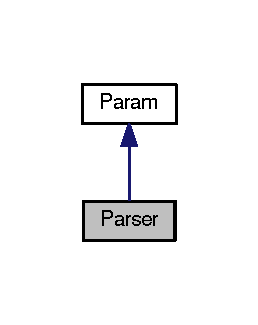
\includegraphics[width=124pt]{classParser__inherit__graph}
\end{center}
\end{figure}


Collaboration diagram for Parser\-:\nopagebreak
\begin{figure}[H]
\begin{center}
\leavevmode
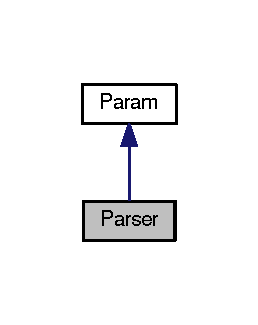
\includegraphics[width=124pt]{classParser__coll__graph}
\end{center}
\end{figure}
\subsection*{Public Member Functions}
\begin{DoxyCompactItemize}
\item 
\hyperlink{classParser_a12234f6cd36b61af4b50c94a179422c1}{Parser} ()
\item 
\hyperlink{classParser_ae3012c947e9d131330b5cf510ba8bc2c}{Parser} (const char $\ast$Input\-File)
\item 
\hyperlink{classParser_a3e658b5917a93a3ef648050d060e3a93}{$\sim$\-Parser} ()
\item 
void \hyperlink{classParser_ae7099218e09ec122508491630f5f6ca0}{add} (char Red\-Line\mbox{[}$\,$\mbox{]})
\end{DoxyCompactItemize}
\subsection*{Private Member Functions}
\begin{DoxyCompactItemize}
\item 
void \hyperlink{classParser_a4c787913235c16c0d2ae774daf25afb6}{Read\-Input\-File} (const char $\ast$Input\-File)
\end{DoxyCompactItemize}
\subsection*{Private Attributes}
\begin{DoxyCompactItemize}
\item 
char \hyperlink{classParser_a2b2cf77a6f8a340790e467557cbc5a12}{type\-\_\-ldelim}
\item 
char \hyperlink{classParser_adfd95f7f5fce9f3d6effd2160ab3b4d3}{type\-\_\-rdelim}
\end{DoxyCompactItemize}
\subsection*{Additional Inherited Members}


\subsection{Constructor \& Destructor Documentation}
\hypertarget{classParser_a12234f6cd36b61af4b50c94a179422c1}{\index{Parser@{Parser}!Parser@{Parser}}
\index{Parser@{Parser}!Parser@{Parser}}
\subsubsection[{Parser}]{\setlength{\rightskip}{0pt plus 5cm}Parser\-::\-Parser (
\begin{DoxyParamCaption}
{}
\end{DoxyParamCaption}
)}}\label{classParser_a12234f6cd36b61af4b50c94a179422c1}
\hypertarget{classParser_ae3012c947e9d131330b5cf510ba8bc2c}{\index{Parser@{Parser}!Parser@{Parser}}
\index{Parser@{Parser}!Parser@{Parser}}
\subsubsection[{Parser}]{\setlength{\rightskip}{0pt plus 5cm}Parser\-::\-Parser (
\begin{DoxyParamCaption}
\item[{const char $\ast$}]{Input\-File}
\end{DoxyParamCaption}
)}}\label{classParser_ae3012c947e9d131330b5cf510ba8bc2c}


References Read\-Input\-File(), type\-\_\-ldelim, and type\-\_\-rdelim.

\hypertarget{classParser_a3e658b5917a93a3ef648050d060e3a93}{\index{Parser@{Parser}!$\sim$\-Parser@{$\sim$\-Parser}}
\index{$\sim$\-Parser@{$\sim$\-Parser}!Parser@{Parser}}
\subsubsection[{$\sim$\-Parser}]{\setlength{\rightskip}{0pt plus 5cm}Parser\-::$\sim$\-Parser (
\begin{DoxyParamCaption}
{}
\end{DoxyParamCaption}
)}}\label{classParser_a3e658b5917a93a3ef648050d060e3a93}


\subsection{Member Function Documentation}
\hypertarget{classParser_ae7099218e09ec122508491630f5f6ca0}{\index{Parser@{Parser}!add@{add}}
\index{add@{add}!Parser@{Parser}}
\subsubsection[{add}]{\setlength{\rightskip}{0pt plus 5cm}void Parser\-::add (
\begin{DoxyParamCaption}
\item[{char}]{Red\-Line\mbox{[}$\,$\mbox{]}}
\end{DoxyParamCaption}
)}}\label{classParser_ae7099218e09ec122508491630f5f6ca0}


References char\-Ptr\-Tovector(), Param\-::\-M, T\-\_\-\-D\-O\-U\-B\-L\-E, T\-\_\-\-I\-N\-T, T\-\_\-\-L\-O\-N\-G, T\-\_\-\-S\-T\-R\-I\-N\-G, T\-\_\-\-V\-E\-C\-T\-O\-R, Type\-Val\-::type, type\-\_\-ldelim, type\-\_\-rdelim, and Type\-Val\-::\-Val.



Referenced by Read\-Input\-File().

\hypertarget{classParser_a4c787913235c16c0d2ae774daf25afb6}{\index{Parser@{Parser}!Read\-Input\-File@{Read\-Input\-File}}
\index{Read\-Input\-File@{Read\-Input\-File}!Parser@{Parser}}
\subsubsection[{Read\-Input\-File}]{\setlength{\rightskip}{0pt plus 5cm}void Parser\-::\-Read\-Input\-File (
\begin{DoxyParamCaption}
\item[{const char $\ast$}]{Input\-File}
\end{DoxyParamCaption}
)\hspace{0.3cm}{\ttfamily [private]}}}\label{classParser_a4c787913235c16c0d2ae774daf25afb6}


References add(), and M\-A\-X\-\_\-\-C\-H\-A\-R\-\_\-\-L\-I\-N\-E.



Referenced by Parser().



\subsection{Field Documentation}
\hypertarget{classParser_a2b2cf77a6f8a340790e467557cbc5a12}{\index{Parser@{Parser}!type\-\_\-ldelim@{type\-\_\-ldelim}}
\index{type\-\_\-ldelim@{type\-\_\-ldelim}!Parser@{Parser}}
\subsubsection[{type\-\_\-ldelim}]{\setlength{\rightskip}{0pt plus 5cm}char Parser\-::type\-\_\-ldelim\hspace{0.3cm}{\ttfamily [private]}}}\label{classParser_a2b2cf77a6f8a340790e467557cbc5a12}


Referenced by add(), and Parser().

\hypertarget{classParser_adfd95f7f5fce9f3d6effd2160ab3b4d3}{\index{Parser@{Parser}!type\-\_\-rdelim@{type\-\_\-rdelim}}
\index{type\-\_\-rdelim@{type\-\_\-rdelim}!Parser@{Parser}}
\subsubsection[{type\-\_\-rdelim}]{\setlength{\rightskip}{0pt plus 5cm}char Parser\-::type\-\_\-rdelim\hspace{0.3cm}{\ttfamily [private]}}}\label{classParser_adfd95f7f5fce9f3d6effd2160ab3b4d3}


Referenced by add(), and Parser().



The documentation for this class was generated from the following files\-:\begin{DoxyCompactItemize}
\item 
/user/0/.\-base/charmont/home/\-Documents/3\-A/\-Projet/pricer\-Monte\-Carlo/src/\hyperlink{parser_8hpp}{parser.\-hpp}\item 
/user/0/.\-base/charmont/home/\-Documents/3\-A/\-Projet/pricer\-Monte\-Carlo/src/\hyperlink{parser_8cpp}{parser.\-cpp}\end{DoxyCompactItemize}

\hypertarget{classTypeVal}{\section{Type\-Val Class Reference}
\label{classTypeVal}\index{Type\-Val@{Type\-Val}}
}


{\ttfamily \#include $<$parser.\-hpp$>$}

\subsection*{Public Member Functions}
\begin{DoxyCompactItemize}
\item 
\hyperlink{classTypeVal_a584555ce9b88dfa20ab05d15980dcaf9}{Type\-Val} ()
\item 
\hyperlink{classTypeVal_a9678b5a8d9ad157f0a813aca8ddd565e}{Type\-Val} (const \hyperlink{classTypeVal}{Type\-Val} \&)
\item 
\hyperlink{classTypeVal_a99d6508946d07b5a4cc7b2419c838445}{$\sim$\-Type\-Val} ()
\item 
\hyperlink{classTypeVal}{Type\-Val} \& \hyperlink{classTypeVal_a001121d22f62c3c895760f23691666e6}{operator=} (const \hyperlink{classTypeVal}{Type\-Val} \&v)
\item 
void \hyperlink{classTypeVal_a5cc7b3e408b42f6ba0c0c6a339c4282e}{print} (const std\-::string \&s) const 
\end{DoxyCompactItemize}
\subsection*{Data Fields}
\begin{DoxyCompactItemize}
\item 
\hyperlink{parser_8hpp_a90856b8fb3f1a65845ffec1ec2884c0f}{T\-\_\-type} \hyperlink{classTypeVal_abd5dd71d2a5e2ce2f3b1f018068108ff}{type}
\item 
boost\-::variant$<$ int, size\-\_\-t, \\*
double, std\-::vector$<$ double $>$\\*
, std\-::string $>$ \hyperlink{classTypeVal_abafd45e0ebbcb8129080cddbea3b3d7b}{Val}
\end{DoxyCompactItemize}
\subsection*{Private Member Functions}
\begin{DoxyCompactItemize}
\item 
{\footnotesize template$<$class Archive $>$ }\\void \hyperlink{classTypeVal_a2278bab9356abb527a4758f32645142d}{serialize} (Archive \&ar, const unsigned int version)
\end{DoxyCompactItemize}
\subsection*{Friends}
\begin{DoxyCompactItemize}
\item 
class \hyperlink{classTypeVal_ac98d07dd8f7b70e16ccb9a01abf56b9c}{boost\-::serialization\-::access}
\end{DoxyCompactItemize}


\subsection{Constructor \& Destructor Documentation}
\hypertarget{classTypeVal_a584555ce9b88dfa20ab05d15980dcaf9}{\index{Type\-Val@{Type\-Val}!Type\-Val@{Type\-Val}}
\index{Type\-Val@{Type\-Val}!TypeVal@{Type\-Val}}
\subsubsection[{Type\-Val}]{\setlength{\rightskip}{0pt plus 5cm}Type\-Val\-::\-Type\-Val (
\begin{DoxyParamCaption}
{}
\end{DoxyParamCaption}
)}}\label{classTypeVal_a584555ce9b88dfa20ab05d15980dcaf9}
\hypertarget{classTypeVal_a9678b5a8d9ad157f0a813aca8ddd565e}{\index{Type\-Val@{Type\-Val}!Type\-Val@{Type\-Val}}
\index{Type\-Val@{Type\-Val}!TypeVal@{Type\-Val}}
\subsubsection[{Type\-Val}]{\setlength{\rightskip}{0pt plus 5cm}Type\-Val\-::\-Type\-Val (
\begin{DoxyParamCaption}
\item[{const {\bf Type\-Val} \&}]{v}
\end{DoxyParamCaption}
)}}\label{classTypeVal_a9678b5a8d9ad157f0a813aca8ddd565e}


References T\-\_\-\-D\-O\-U\-B\-L\-E, T\-\_\-\-I\-N\-T, T\-\_\-\-L\-O\-N\-G, T\-\_\-\-S\-T\-R\-I\-N\-G, T\-\_\-\-V\-E\-C\-T\-O\-R, type, and Val.

\hypertarget{classTypeVal_a99d6508946d07b5a4cc7b2419c838445}{\index{Type\-Val@{Type\-Val}!$\sim$\-Type\-Val@{$\sim$\-Type\-Val}}
\index{$\sim$\-Type\-Val@{$\sim$\-Type\-Val}!TypeVal@{Type\-Val}}
\subsubsection[{$\sim$\-Type\-Val}]{\setlength{\rightskip}{0pt plus 5cm}Type\-Val\-::$\sim$\-Type\-Val (
\begin{DoxyParamCaption}
{}
\end{DoxyParamCaption}
)}}\label{classTypeVal_a99d6508946d07b5a4cc7b2419c838445}


\subsection{Member Function Documentation}
\hypertarget{classTypeVal_a001121d22f62c3c895760f23691666e6}{\index{Type\-Val@{Type\-Val}!operator=@{operator=}}
\index{operator=@{operator=}!TypeVal@{Type\-Val}}
\subsubsection[{operator=}]{\setlength{\rightskip}{0pt plus 5cm}{\bf Type\-Val} \& Type\-Val\-::operator= (
\begin{DoxyParamCaption}
\item[{const {\bf Type\-Val} \&}]{v}
\end{DoxyParamCaption}
)}}\label{classTypeVal_a001121d22f62c3c895760f23691666e6}


References T\-\_\-\-D\-O\-U\-B\-L\-E, T\-\_\-\-I\-N\-T, T\-\_\-\-L\-O\-N\-G, T\-\_\-\-S\-T\-R\-I\-N\-G, T\-\_\-\-V\-E\-C\-T\-O\-R, type, and Val.

\hypertarget{classTypeVal_a5cc7b3e408b42f6ba0c0c6a339c4282e}{\index{Type\-Val@{Type\-Val}!print@{print}}
\index{print@{print}!TypeVal@{Type\-Val}}
\subsubsection[{print}]{\setlength{\rightskip}{0pt plus 5cm}void Type\-Val\-::print (
\begin{DoxyParamCaption}
\item[{const std\-::string \&}]{s}
\end{DoxyParamCaption}
) const}}\label{classTypeVal_a5cc7b3e408b42f6ba0c0c6a339c4282e}


References T\-\_\-\-D\-O\-U\-B\-L\-E, T\-\_\-\-I\-N\-T, T\-\_\-\-L\-O\-N\-G, T\-\_\-\-S\-T\-R\-I\-N\-G, and T\-\_\-\-V\-E\-C\-T\-O\-R.

\hypertarget{classTypeVal_a2278bab9356abb527a4758f32645142d}{\index{Type\-Val@{Type\-Val}!serialize@{serialize}}
\index{serialize@{serialize}!TypeVal@{Type\-Val}}
\subsubsection[{serialize}]{\setlength{\rightskip}{0pt plus 5cm}template$<$class Archive $>$ void Type\-Val\-::serialize (
\begin{DoxyParamCaption}
\item[{Archive \&}]{ar, }
\item[{const unsigned int}]{version}
\end{DoxyParamCaption}
)\hspace{0.3cm}{\ttfamily [inline]}, {\ttfamily [private]}}}\label{classTypeVal_a2278bab9356abb527a4758f32645142d}


References type, and Val.



\subsection{Friends And Related Function Documentation}
\hypertarget{classTypeVal_ac98d07dd8f7b70e16ccb9a01abf56b9c}{\index{Type\-Val@{Type\-Val}!boost\-::serialization\-::access@{boost\-::serialization\-::access}}
\index{boost\-::serialization\-::access@{boost\-::serialization\-::access}!TypeVal@{Type\-Val}}
\subsubsection[{boost\-::serialization\-::access}]{\setlength{\rightskip}{0pt plus 5cm}friend class boost\-::serialization\-::access\hspace{0.3cm}{\ttfamily [friend]}}}\label{classTypeVal_ac98d07dd8f7b70e16ccb9a01abf56b9c}


\subsection{Field Documentation}
\hypertarget{classTypeVal_abd5dd71d2a5e2ce2f3b1f018068108ff}{\index{Type\-Val@{Type\-Val}!type@{type}}
\index{type@{type}!TypeVal@{Type\-Val}}
\subsubsection[{type}]{\setlength{\rightskip}{0pt plus 5cm}{\bf T\-\_\-type} Type\-Val\-::type}}\label{classTypeVal_abd5dd71d2a5e2ce2f3b1f018068108ff}


Referenced by Parser\-::add(), Param\-::insert(), operator=(), serialize(), and Type\-Val().

\hypertarget{classTypeVal_abafd45e0ebbcb8129080cddbea3b3d7b}{\index{Type\-Val@{Type\-Val}!Val@{Val}}
\index{Val@{Val}!TypeVal@{Type\-Val}}
\subsubsection[{Val}]{\setlength{\rightskip}{0pt plus 5cm}boost\-::variant$<$int, size\-\_\-t, double, std\-::vector$<$double$>$, std\-::string$>$ Type\-Val\-::\-Val}}\label{classTypeVal_abafd45e0ebbcb8129080cddbea3b3d7b}


Referenced by Parser\-::add(), Param\-::insert(), operator=(), serialize(), and Type\-Val().



The documentation for this class was generated from the following files\-:\begin{DoxyCompactItemize}
\item 
/user/0/.\-base/charmont/home/\-Documents/3\-A/\-Projet/pricer\-Monte\-Carlo/src/\hyperlink{parser_8hpp}{parser.\-hpp}\item 
/user/0/.\-base/charmont/home/\-Documents/3\-A/\-Projet/pricer\-Monte\-Carlo/src/\hyperlink{parser_8cpp}{parser.\-cpp}\end{DoxyCompactItemize}

\chapter{File Documentation}
\hypertarget{BlackScholesModel_8cpp}{\section{/user/2/.base/margueed/home/pricer\-Monte\-Carlo/src/\-Black\-Scholes\-Model.cpp File Reference}
\label{BlackScholesModel_8cpp}\index{/user/2/.\-base/margueed/home/pricer\-Monte\-Carlo/src/\-Black\-Scholes\-Model.\-cpp@{/user/2/.\-base/margueed/home/pricer\-Monte\-Carlo/src/\-Black\-Scholes\-Model.\-cpp}}
}
{\ttfamily \#include \char`\"{}Black\-Scholes\-Model.\-hpp\char`\"{}}\\*
{\ttfamily \#include $<$cmath$>$}\\*
{\ttfamily \#include $<$iostream$>$}\\*
Include dependency graph for Black\-Scholes\-Model.\-cpp\-:
\nopagebreak
\begin{figure}[H]
\begin{center}
\leavevmode
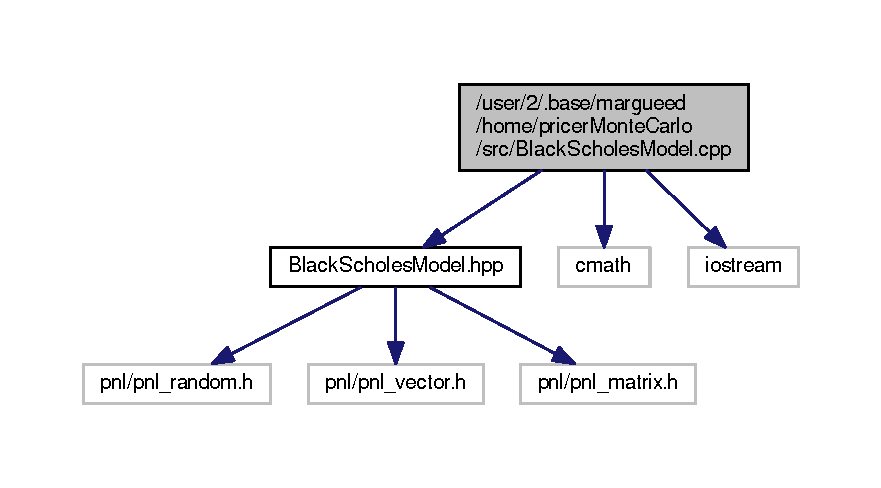
\includegraphics[width=350pt]{BlackScholesModel_8cpp__incl}
\end{center}
\end{figure}

\hypertarget{BlackScholesModel_8hpp}{\section{/user/2/.base/margueed/home/pricer\-Monte\-Carlo/src/\-Black\-Scholes\-Model.hpp File Reference}
\label{BlackScholesModel_8hpp}\index{/user/2/.\-base/margueed/home/pricer\-Monte\-Carlo/src/\-Black\-Scholes\-Model.\-hpp@{/user/2/.\-base/margueed/home/pricer\-Monte\-Carlo/src/\-Black\-Scholes\-Model.\-hpp}}
}
{\ttfamily \#include \char`\"{}pnl/pnl\-\_\-random.\-h\char`\"{}}\\*
{\ttfamily \#include \char`\"{}pnl/pnl\-\_\-vector.\-h\char`\"{}}\\*
{\ttfamily \#include \char`\"{}pnl/pnl\-\_\-matrix.\-h\char`\"{}}\\*
Include dependency graph for Black\-Scholes\-Model.\-hpp\-:
\nopagebreak
\begin{figure}[H]
\begin{center}
\leavevmode
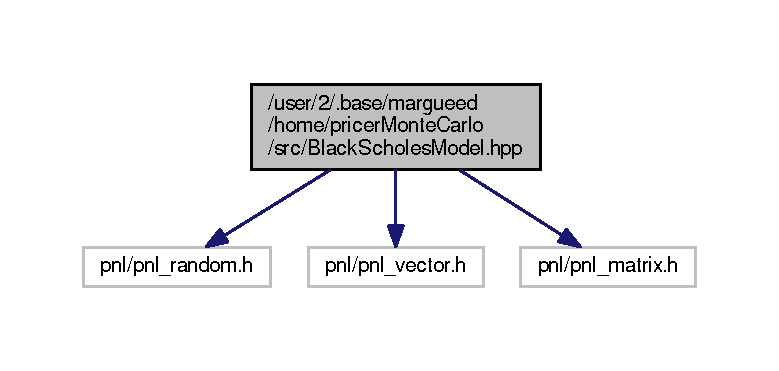
\includegraphics[width=350pt]{BlackScholesModel_8hpp__incl}
\end{center}
\end{figure}
This graph shows which files directly or indirectly include this file\-:
\nopagebreak
\begin{figure}[H]
\begin{center}
\leavevmode
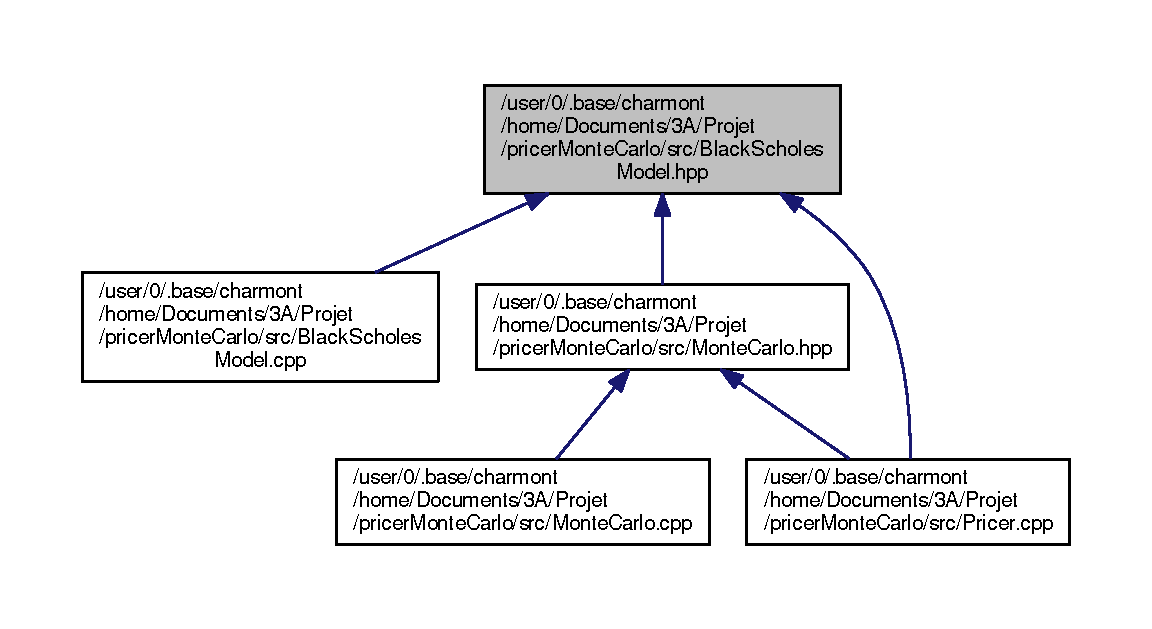
\includegraphics[width=350pt]{BlackScholesModel_8hpp__dep__incl}
\end{center}
\end{figure}
\subsection*{Data Structures}
\begin{DoxyCompactItemize}
\item 
class \hyperlink{classBlackScholesModel}{Black\-Scholes\-Model}
\begin{DoxyCompactList}\small\item\em Modèle de Black Scholes. \end{DoxyCompactList}\end{DoxyCompactItemize}

\hypertarget{MonteCarlo_8cpp}{\section{/user/2/.base/margueed/home/pricer\-Monte\-Carlo/src/\-Monte\-Carlo.cpp File Reference}
\label{MonteCarlo_8cpp}\index{/user/2/.\-base/margueed/home/pricer\-Monte\-Carlo/src/\-Monte\-Carlo.\-cpp@{/user/2/.\-base/margueed/home/pricer\-Monte\-Carlo/src/\-Monte\-Carlo.\-cpp}}
}
{\ttfamily \#include \char`\"{}Monte\-Carlo.\-hpp\char`\"{}}\\*
{\ttfamily \#include $<$iostream$>$}\\*
{\ttfamily \#include $<$ctime$>$}\\*
{\ttfamily \#include $<$cmath$>$}\\*
{\ttfamily \#include \char`\"{}pnl/pnl\-\_\-random.\-h\char`\"{}}\\*
{\ttfamily \#include \char`\"{}pnl/pnl\-\_\-vector.\-h\char`\"{}}\\*
Include dependency graph for Monte\-Carlo.\-cpp\-:
\nopagebreak
\begin{figure}[H]
\begin{center}
\leavevmode
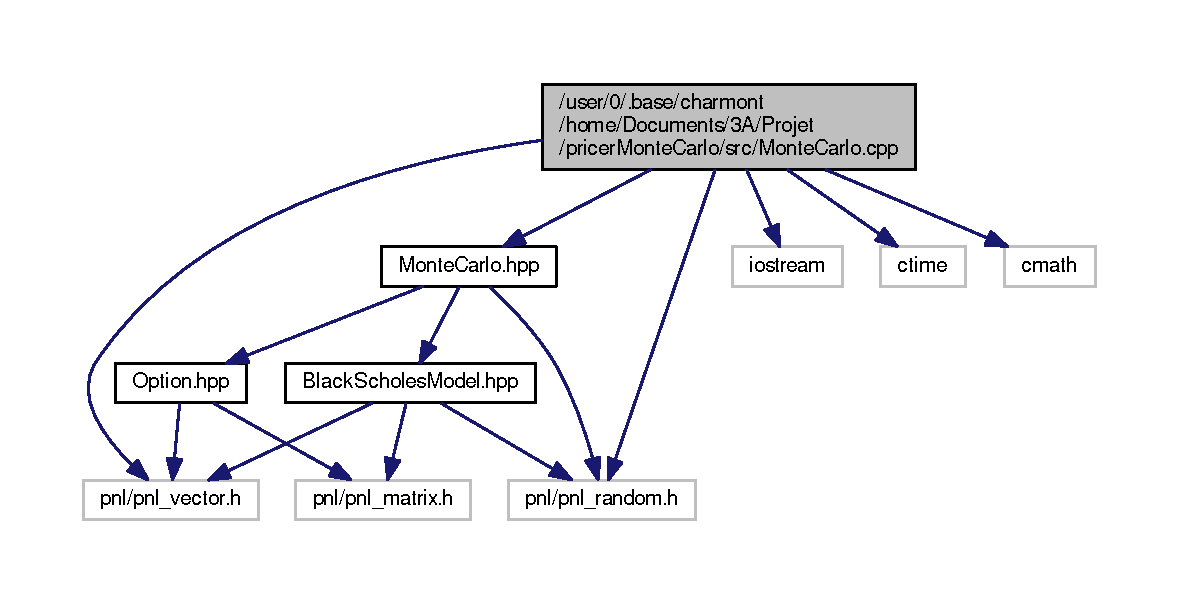
\includegraphics[width=350pt]{MonteCarlo_8cpp__incl}
\end{center}
\end{figure}

\hypertarget{MonteCarlo_8hpp}{\section{/user/2/.base/margueed/home/pricer\-Monte\-Carlo/src/\-Monte\-Carlo.hpp File Reference}
\label{MonteCarlo_8hpp}\index{/user/2/.\-base/margueed/home/pricer\-Monte\-Carlo/src/\-Monte\-Carlo.\-hpp@{/user/2/.\-base/margueed/home/pricer\-Monte\-Carlo/src/\-Monte\-Carlo.\-hpp}}
}
{\ttfamily \#include \char`\"{}Option.\-hpp\char`\"{}}\\*
{\ttfamily \#include \char`\"{}Black\-Scholes\-Model.\-hpp\char`\"{}}\\*
{\ttfamily \#include \char`\"{}pnl/pnl\-\_\-random.\-h\char`\"{}}\\*
Include dependency graph for Monte\-Carlo.\-hpp\-:
\nopagebreak
\begin{figure}[H]
\begin{center}
\leavevmode
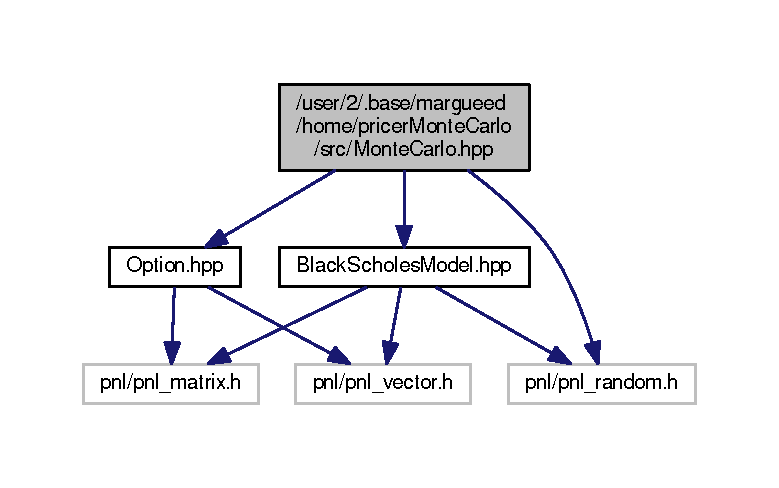
\includegraphics[width=350pt]{MonteCarlo_8hpp__incl}
\end{center}
\end{figure}
This graph shows which files directly or indirectly include this file\-:
\nopagebreak
\begin{figure}[H]
\begin{center}
\leavevmode
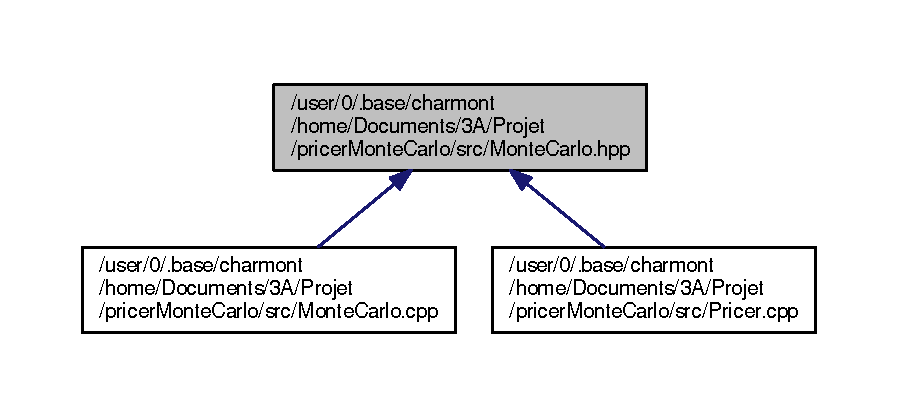
\includegraphics[width=338pt]{MonteCarlo_8hpp__dep__incl}
\end{center}
\end{figure}
\subsection*{Data Structures}
\begin{DoxyCompactItemize}
\item 
class \hyperlink{classMonteCarlo}{Monte\-Carlo}
\end{DoxyCompactItemize}

\hypertarget{Option_8cpp}{\section{/user/2/.base/margueed/home/pricer\-Monte\-Carlo/src/\-Option.cpp File Reference}
\label{Option_8cpp}\index{/user/2/.\-base/margueed/home/pricer\-Monte\-Carlo/src/\-Option.\-cpp@{/user/2/.\-base/margueed/home/pricer\-Monte\-Carlo/src/\-Option.\-cpp}}
}
{\ttfamily \#include \char`\"{}Option.\-hpp\char`\"{}}\\*
Include dependency graph for Option.\-cpp\-:
\nopagebreak
\begin{figure}[H]
\begin{center}
\leavevmode
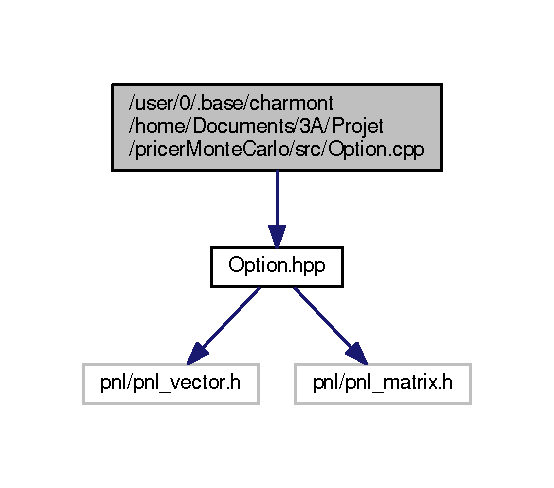
\includegraphics[width=266pt]{Option_8cpp__incl}
\end{center}
\end{figure}

\hypertarget{Option_8hpp}{\section{/user/2/.base/margueed/home/pricer\-Monte\-Carlo/src/\-Option.hpp File Reference}
\label{Option_8hpp}\index{/user/2/.\-base/margueed/home/pricer\-Monte\-Carlo/src/\-Option.\-hpp@{/user/2/.\-base/margueed/home/pricer\-Monte\-Carlo/src/\-Option.\-hpp}}
}
{\ttfamily \#include \char`\"{}pnl/pnl\-\_\-vector.\-h\char`\"{}}\\*
{\ttfamily \#include \char`\"{}pnl/pnl\-\_\-matrix.\-h\char`\"{}}\\*
Include dependency graph for Option.\-hpp\-:
\nopagebreak
\begin{figure}[H]
\begin{center}
\leavevmode
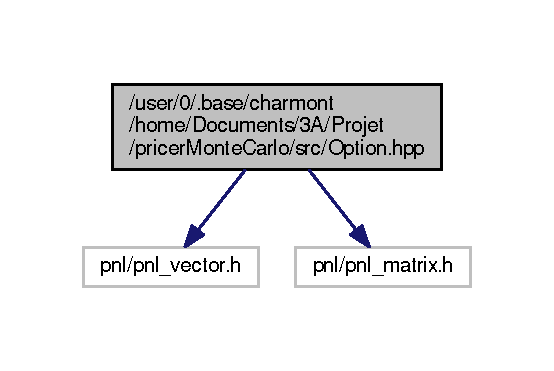
\includegraphics[width=266pt]{Option_8hpp__incl}
\end{center}
\end{figure}
This graph shows which files directly or indirectly include this file\-:
\nopagebreak
\begin{figure}[H]
\begin{center}
\leavevmode
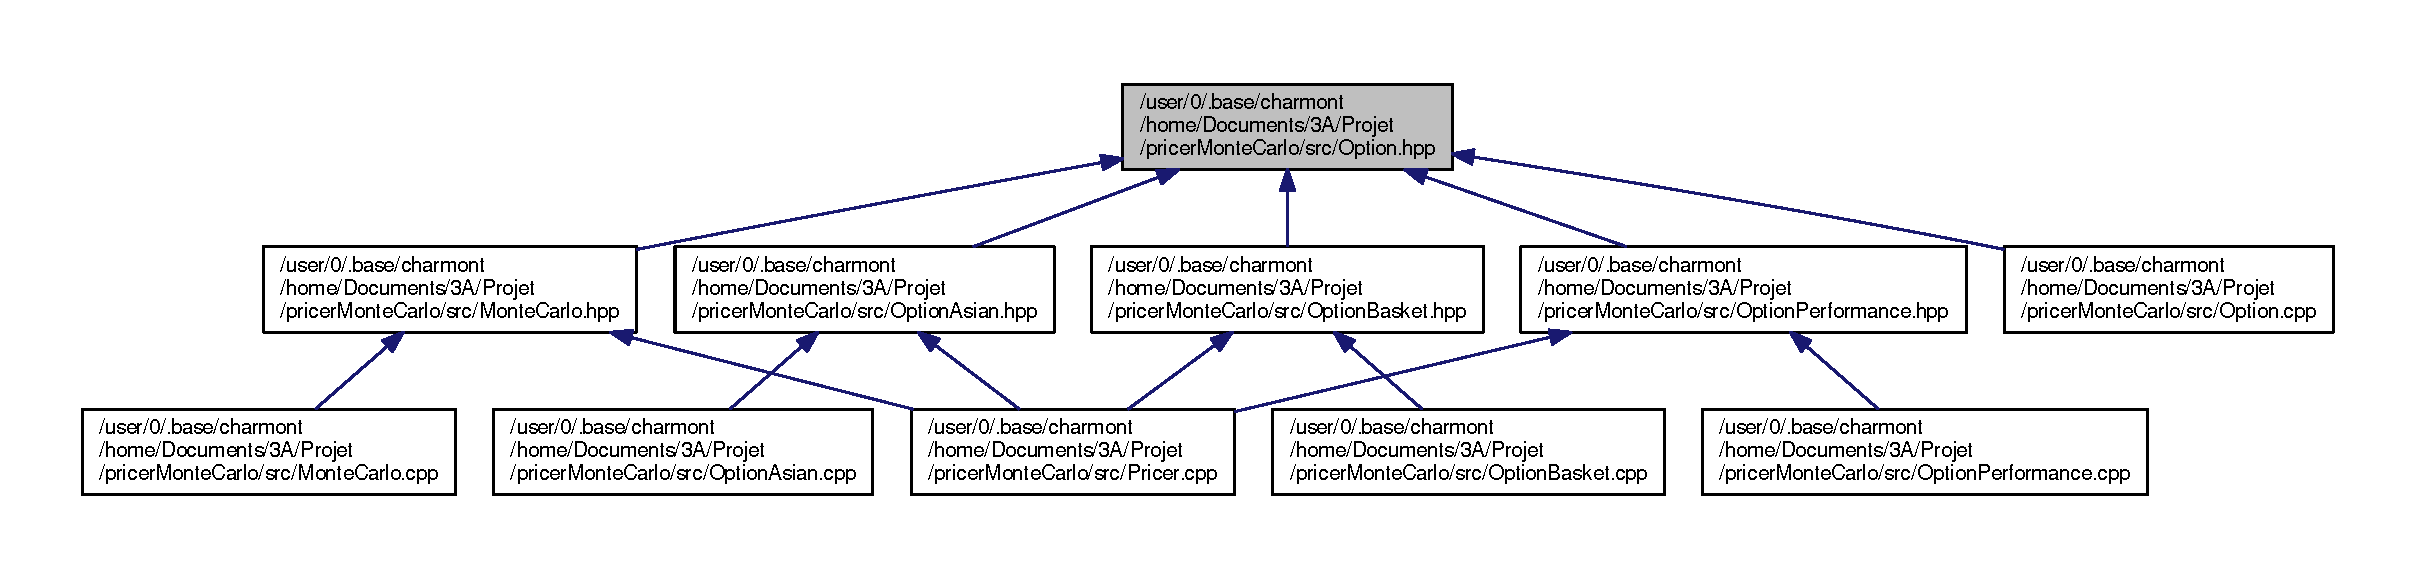
\includegraphics[width=350pt]{Option_8hpp__dep__incl}
\end{center}
\end{figure}
\subsection*{Data Structures}
\begin{DoxyCompactItemize}
\item 
class \hyperlink{classOption}{Option}
\begin{DoxyCompactList}\small\item\em Classe \hyperlink{classOption}{Option} abstraite. \end{DoxyCompactList}\end{DoxyCompactItemize}

\hypertarget{OptionAsian_8cpp}{\section{/user/2/.base/margueed/home/pricer\-Monte\-Carlo/src/\-Option\-Asian.cpp File Reference}
\label{OptionAsian_8cpp}\index{/user/2/.\-base/margueed/home/pricer\-Monte\-Carlo/src/\-Option\-Asian.\-cpp@{/user/2/.\-base/margueed/home/pricer\-Monte\-Carlo/src/\-Option\-Asian.\-cpp}}
}
{\ttfamily \#include \char`\"{}Option\-Asian.\-hpp\char`\"{}}\\*
Include dependency graph for Option\-Asian.\-cpp\-:
\nopagebreak
\begin{figure}[H]
\begin{center}
\leavevmode
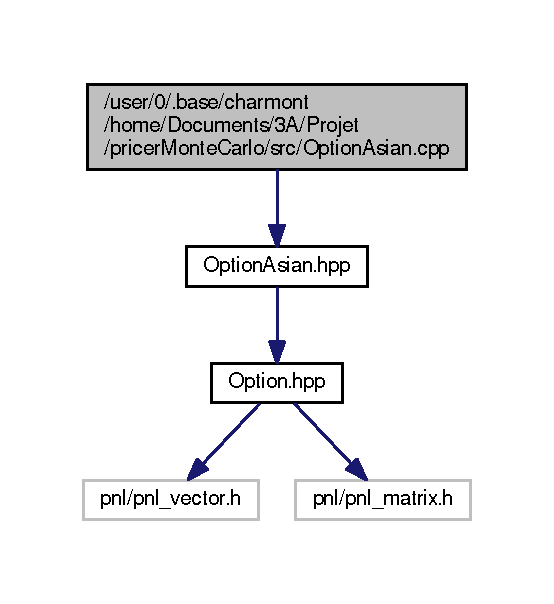
\includegraphics[width=266pt]{OptionAsian_8cpp__incl}
\end{center}
\end{figure}

\hypertarget{OptionAsian_8hpp}{\section{/user/2/.base/margueed/home/pricer\-Monte\-Carlo/src/\-Option\-Asian.hpp File Reference}
\label{OptionAsian_8hpp}\index{/user/2/.\-base/margueed/home/pricer\-Monte\-Carlo/src/\-Option\-Asian.\-hpp@{/user/2/.\-base/margueed/home/pricer\-Monte\-Carlo/src/\-Option\-Asian.\-hpp}}
}
{\ttfamily \#include \char`\"{}Option.\-hpp\char`\"{}}\\*
Include dependency graph for Option\-Asian.\-hpp\-:
\nopagebreak
\begin{figure}[H]
\begin{center}
\leavevmode
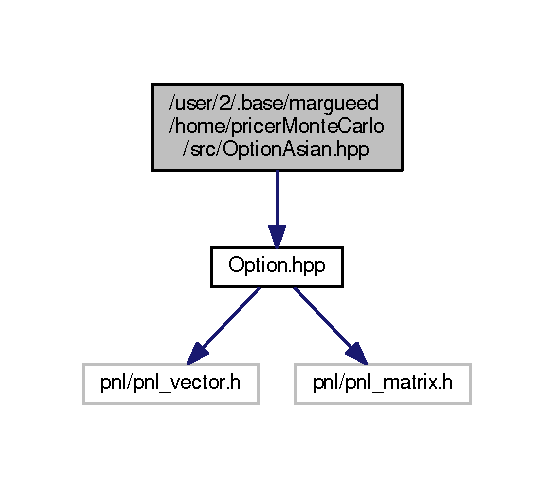
\includegraphics[width=266pt]{OptionAsian_8hpp__incl}
\end{center}
\end{figure}
This graph shows which files directly or indirectly include this file\-:
\nopagebreak
\begin{figure}[H]
\begin{center}
\leavevmode
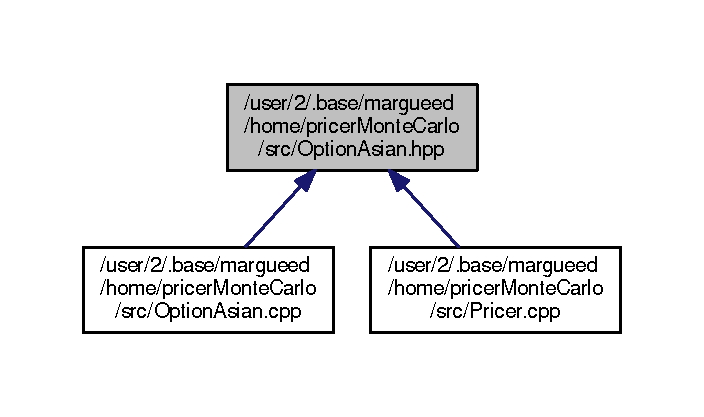
\includegraphics[width=338pt]{OptionAsian_8hpp__dep__incl}
\end{center}
\end{figure}
\subsection*{Data Structures}
\begin{DoxyCompactItemize}
\item 
class \hyperlink{classOptionAsian}{Option\-Asian}
\end{DoxyCompactItemize}

\hypertarget{OptionBasket_8cpp}{\section{/user/0/.base/charmont/home/\-Documents/3\-A/\-Projet/pricer\-Monte\-Carlo/src/\-Option\-Basket.cpp File Reference}
\label{OptionBasket_8cpp}\index{/user/0/.\-base/charmont/home/\-Documents/3\-A/\-Projet/pricer\-Monte\-Carlo/src/\-Option\-Basket.\-cpp@{/user/0/.\-base/charmont/home/\-Documents/3\-A/\-Projet/pricer\-Monte\-Carlo/src/\-Option\-Basket.\-cpp}}
}
{\ttfamily \#include \char`\"{}Option\-Basket.\-hpp\char`\"{}}\\*
Include dependency graph for Option\-Basket.\-cpp\-:
\nopagebreak
\begin{figure}[H]
\begin{center}
\leavevmode
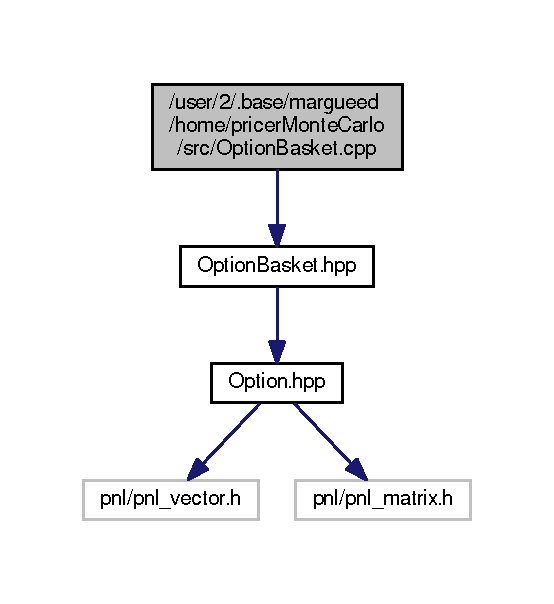
\includegraphics[width=268pt]{OptionBasket_8cpp__incl}
\end{center}
\end{figure}

\hypertarget{OptionBasket_8hpp}{\section{/user/2/.base/margueed/home/pricer\-Monte\-Carlo/src/\-Option\-Basket.hpp File Reference}
\label{OptionBasket_8hpp}\index{/user/2/.\-base/margueed/home/pricer\-Monte\-Carlo/src/\-Option\-Basket.\-hpp@{/user/2/.\-base/margueed/home/pricer\-Monte\-Carlo/src/\-Option\-Basket.\-hpp}}
}
{\ttfamily \#include \char`\"{}Option.\-hpp\char`\"{}}\\*
Include dependency graph for Option\-Basket.\-hpp\-:
\nopagebreak
\begin{figure}[H]
\begin{center}
\leavevmode
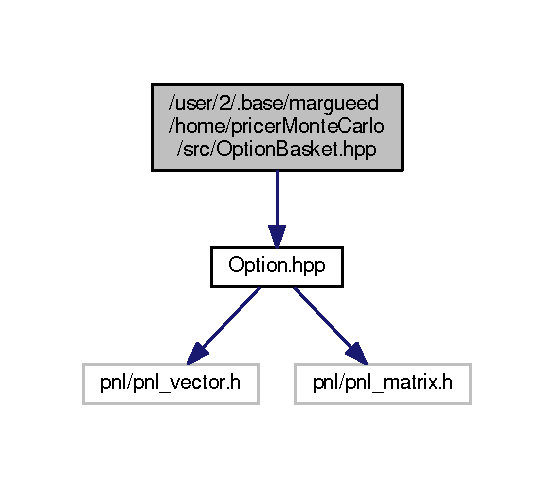
\includegraphics[width=266pt]{OptionBasket_8hpp__incl}
\end{center}
\end{figure}
This graph shows which files directly or indirectly include this file\-:
\nopagebreak
\begin{figure}[H]
\begin{center}
\leavevmode
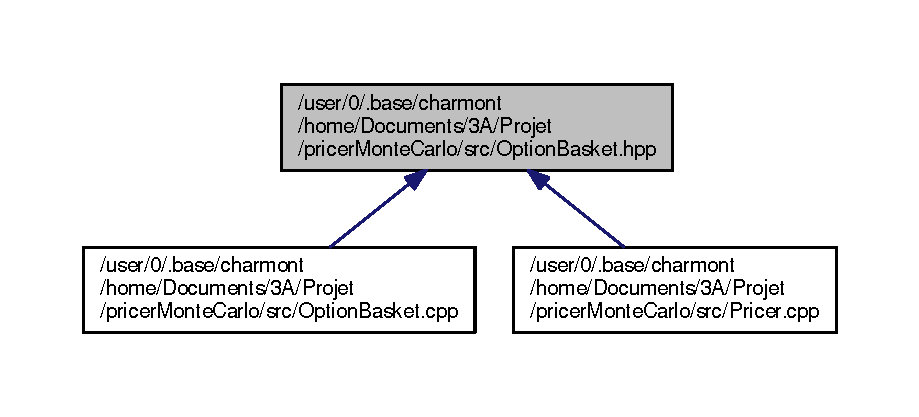
\includegraphics[width=338pt]{OptionBasket_8hpp__dep__incl}
\end{center}
\end{figure}
\subsection*{Data Structures}
\begin{DoxyCompactItemize}
\item 
class \hyperlink{classOptionBasket}{Option\-Basket}
\end{DoxyCompactItemize}

\hypertarget{OptionPerformance_8cpp}{\section{/user/0/.base/charmont/home/\-Documents/3\-A/\-Projet/pricer\-Monte\-Carlo/src/\-Option\-Performance.cpp File Reference}
\label{OptionPerformance_8cpp}\index{/user/0/.\-base/charmont/home/\-Documents/3\-A/\-Projet/pricer\-Monte\-Carlo/src/\-Option\-Performance.\-cpp@{/user/0/.\-base/charmont/home/\-Documents/3\-A/\-Projet/pricer\-Monte\-Carlo/src/\-Option\-Performance.\-cpp}}
}
{\ttfamily \#include \char`\"{}Option\-Performance.\-hpp\char`\"{}}\\*
Include dependency graph for Option\-Performance.\-cpp\-:
\nopagebreak
\begin{figure}[H]
\begin{center}
\leavevmode
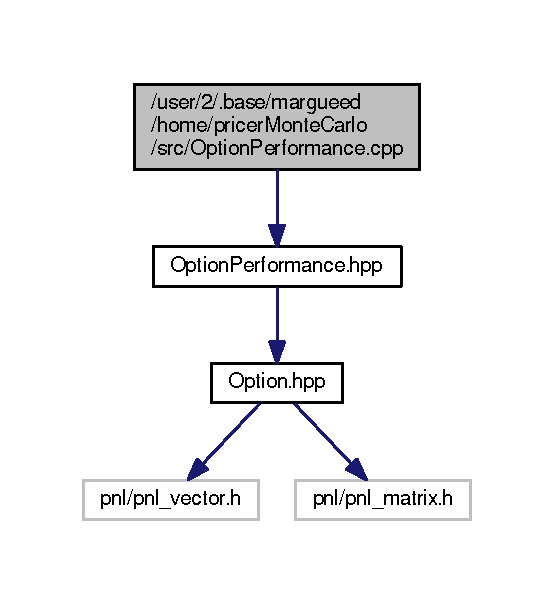
\includegraphics[width=294pt]{OptionPerformance_8cpp__incl}
\end{center}
\end{figure}

\hypertarget{OptionPerformance_8hpp}{\section{/user/0/.base/charmont/home/\-Documents/3\-A/\-Projet/pricer\-Monte\-Carlo/src/\-Option\-Performance.hpp File Reference}
\label{OptionPerformance_8hpp}\index{/user/0/.\-base/charmont/home/\-Documents/3\-A/\-Projet/pricer\-Monte\-Carlo/src/\-Option\-Performance.\-hpp@{/user/0/.\-base/charmont/home/\-Documents/3\-A/\-Projet/pricer\-Monte\-Carlo/src/\-Option\-Performance.\-hpp}}
}
{\ttfamily \#include \char`\"{}Option.\-hpp\char`\"{}}\\*
Include dependency graph for Option\-Performance.\-hpp\-:
\nopagebreak
\begin{figure}[H]
\begin{center}
\leavevmode
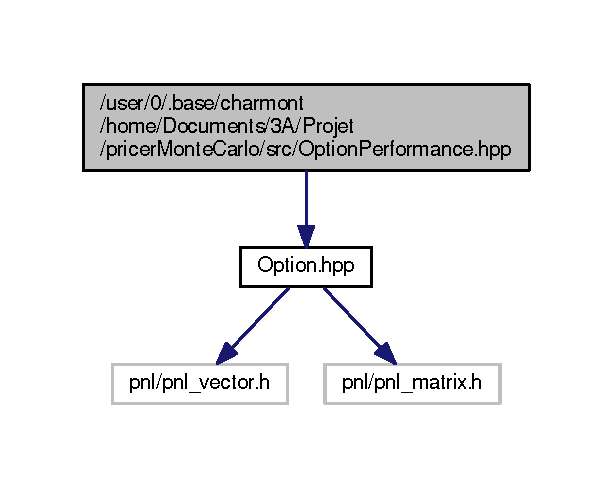
\includegraphics[width=294pt]{OptionPerformance_8hpp__incl}
\end{center}
\end{figure}
This graph shows which files directly or indirectly include this file\-:
\nopagebreak
\begin{figure}[H]
\begin{center}
\leavevmode
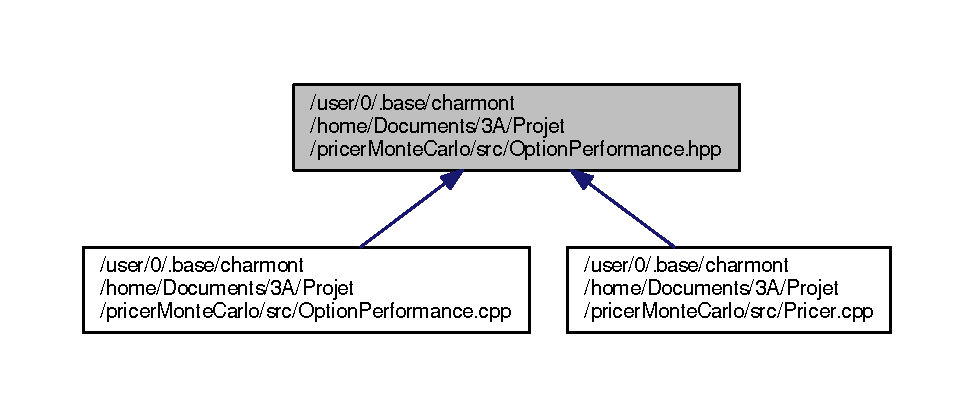
\includegraphics[width=350pt]{OptionPerformance_8hpp__dep__incl}
\end{center}
\end{figure}
\subsection*{Data Structures}
\begin{DoxyCompactItemize}
\item 
class \hyperlink{classOptionPerformance}{Option\-Performance}
\end{DoxyCompactItemize}

\hypertarget{parser_8cpp}{\section{/user/0/.base/charmont/home/\-Documents/3\-A/\-Projet/pricer\-Monte\-Carlo/src/parser.cpp File Reference}
\label{parser_8cpp}\index{/user/0/.\-base/charmont/home/\-Documents/3\-A/\-Projet/pricer\-Monte\-Carlo/src/parser.\-cpp@{/user/0/.\-base/charmont/home/\-Documents/3\-A/\-Projet/pricer\-Monte\-Carlo/src/parser.\-cpp}}
}
{\ttfamily \#include $<$iostream$>$}\\*
{\ttfamily \#include $<$cstdlib$>$}\\*
{\ttfamily \#include $<$cstring$>$}\\*
{\ttfamily \#include $<$algorithm$>$}\\*
{\ttfamily \#include \char`\"{}parser.\-hpp\char`\"{}}\\*
Include dependency graph for parser.\-cpp\-:
\nopagebreak
\begin{figure}[H]
\begin{center}
\leavevmode
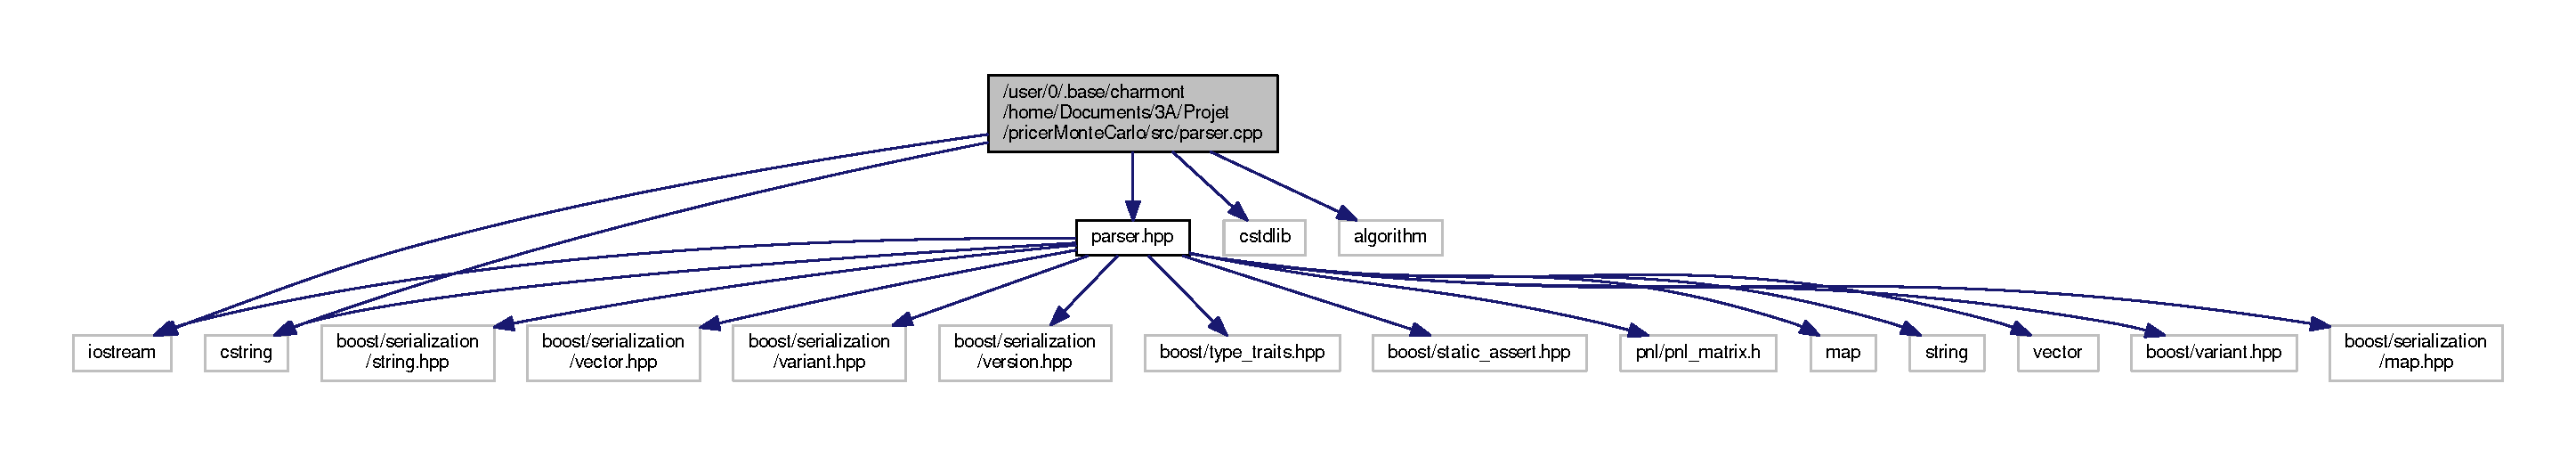
\includegraphics[width=350pt]{parser_8cpp__incl}
\end{center}
\end{figure}
\subsection*{Functions}
\begin{DoxyCompactItemize}
\item 
{\footnotesize template$<$typename T $>$ }\\std\-::ostream \& \hyperlink{parser_8cpp_a752c44978f0f5abde8919968032102bb}{operator$<$$<$} (std\-::ostream \&out, const std\-::vector$<$ T $>$ \&v)
\item 
static vector$<$ double $>$ \hyperlink{parser_8cpp_a269d1c6bbb5f10eb3500e178ec319866}{char\-Ptr\-Tovector} (const char $\ast$s)
\end{DoxyCompactItemize}


\subsection{Function Documentation}
\hypertarget{parser_8cpp_a269d1c6bbb5f10eb3500e178ec319866}{\index{parser.\-cpp@{parser.\-cpp}!char\-Ptr\-Tovector@{char\-Ptr\-Tovector}}
\index{char\-Ptr\-Tovector@{char\-Ptr\-Tovector}!parser.cpp@{parser.\-cpp}}
\subsubsection[{char\-Ptr\-Tovector}]{\setlength{\rightskip}{0pt plus 5cm}static vector$<$double$>$ char\-Ptr\-Tovector (
\begin{DoxyParamCaption}
\item[{const char $\ast$}]{s}
\end{DoxyParamCaption}
)\hspace{0.3cm}{\ttfamily [static]}}}\label{parser_8cpp_a269d1c6bbb5f10eb3500e178ec319866}


Referenced by Parser\-::add().

\hypertarget{parser_8cpp_a752c44978f0f5abde8919968032102bb}{\index{parser.\-cpp@{parser.\-cpp}!operator$<$$<$@{operator$<$$<$}}
\index{operator$<$$<$@{operator$<$$<$}!parser.cpp@{parser.\-cpp}}
\subsubsection[{operator$<$$<$}]{\setlength{\rightskip}{0pt plus 5cm}template$<$typename T $>$ std\-::ostream\& operator$<$$<$ (
\begin{DoxyParamCaption}
\item[{std\-::ostream \&}]{out, }
\item[{const std\-::vector$<$ T $>$ \&}]{v}
\end{DoxyParamCaption}
)}}\label{parser_8cpp_a752c44978f0f5abde8919968032102bb}

\hypertarget{parser_8hpp}{\section{/user/0/.base/charmont/home/\-Documents/3\-A/\-Projet/pricer\-Monte\-Carlo/src/parser.hpp File Reference}
\label{parser_8hpp}\index{/user/0/.\-base/charmont/home/\-Documents/3\-A/\-Projet/pricer\-Monte\-Carlo/src/parser.\-hpp@{/user/0/.\-base/charmont/home/\-Documents/3\-A/\-Projet/pricer\-Monte\-Carlo/src/parser.\-hpp}}
}
{\ttfamily \#include \char`\"{}pnl/pnl\-\_\-matrix.\-h\char`\"{}}\\*
{\ttfamily \#include $<$iostream$>$}\\*
{\ttfamily \#include $<$map$>$}\\*
{\ttfamily \#include $<$string$>$}\\*
{\ttfamily \#include $<$vector$>$}\\*
{\ttfamily \#include $<$cstring$>$}\\*
{\ttfamily \#include $<$boost/variant.\-hpp$>$}\\*
{\ttfamily \#include $<$boost/serialization/map.\-hpp$>$}\\*
{\ttfamily \#include $<$boost/serialization/string.\-hpp$>$}\\*
{\ttfamily \#include $<$boost/serialization/vector.\-hpp$>$}\\*
{\ttfamily \#include $<$boost/serialization/variant.\-hpp$>$}\\*
{\ttfamily \#include $<$boost/serialization/version.\-hpp$>$}\\*
{\ttfamily \#include $<$boost/type\-\_\-traits.\-hpp$>$}\\*
{\ttfamily \#include $<$boost/static\-\_\-assert.\-hpp$>$}\\*
Include dependency graph for parser.\-hpp\-:
\nopagebreak
\begin{figure}[H]
\begin{center}
\leavevmode
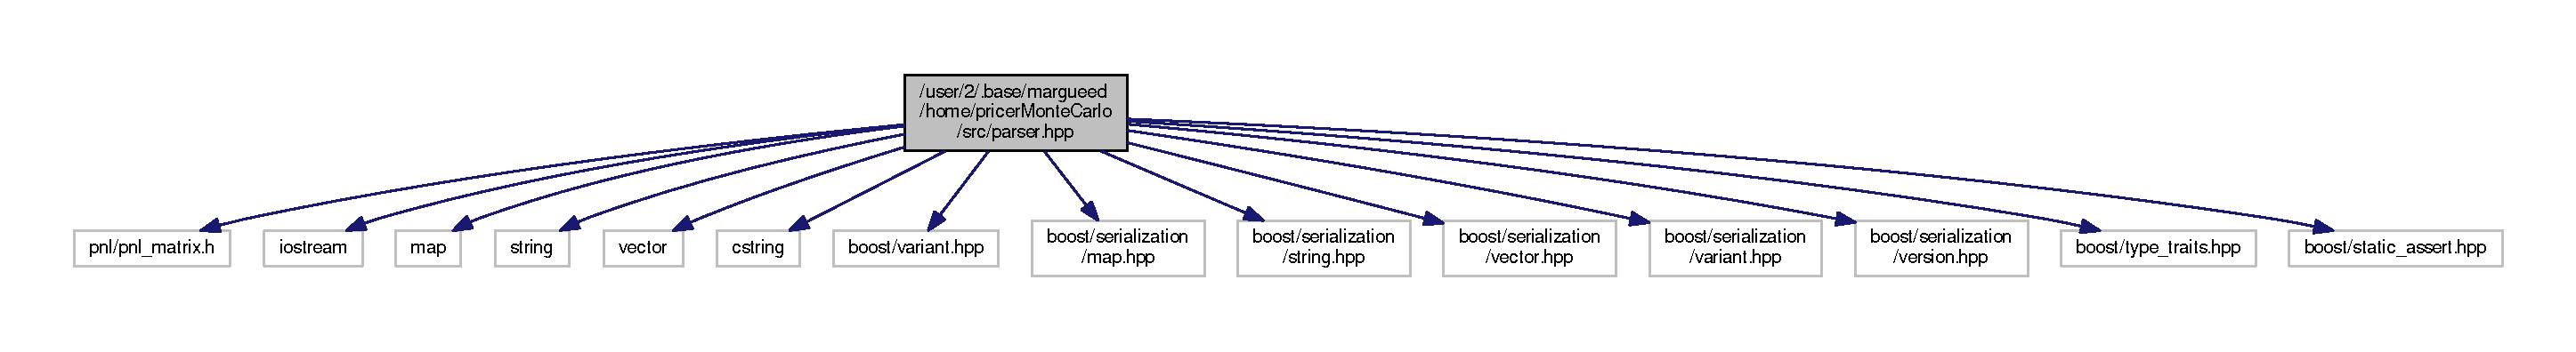
\includegraphics[width=350pt]{parser_8hpp__incl}
\end{center}
\end{figure}
This graph shows which files directly or indirectly include this file\-:
\nopagebreak
\begin{figure}[H]
\begin{center}
\leavevmode
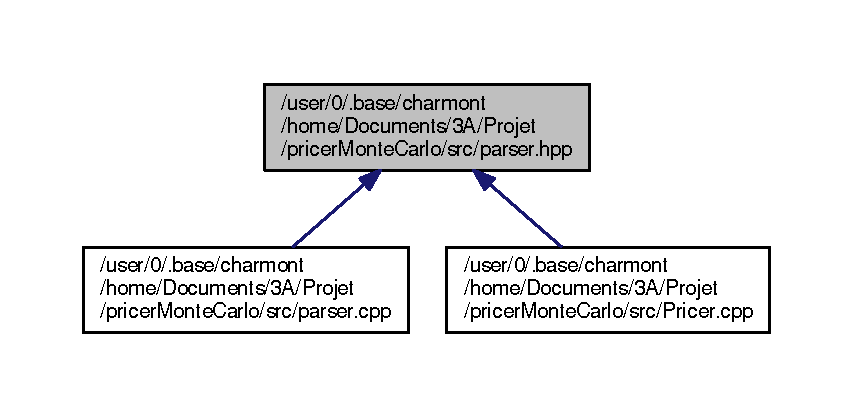
\includegraphics[width=350pt]{parser_8hpp__dep__incl}
\end{center}
\end{figure}
\subsection*{Data Structures}
\begin{DoxyCompactItemize}
\item 
class \hyperlink{classTypeVal}{Type\-Val}
\item 
struct \hyperlink{structcomp}{comp}
\item 
class \hyperlink{classParam}{Param}
\item 
class \hyperlink{classParser}{Parser}
\end{DoxyCompactItemize}
\subsection*{Macros}
\begin{DoxyCompactItemize}
\item 
\#define \hyperlink{parser_8hpp_a3bcbc3ff314d166a1887c5a4ea3e2d1b}{M\-A\-X\-\_\-\-C\-H\-A\-R\-\_\-\-L\-I\-N\-E}~1024
\end{DoxyCompactItemize}
\subsection*{Typedefs}
\begin{DoxyCompactItemize}
\item 
typedef std\-::map$<$ std\-::string, \\*
\hyperlink{classTypeVal}{Type\-Val}, \hyperlink{structcomp}{comp} $>$ \hyperlink{parser_8hpp_a77c3bfcf208503ef5164669afcd00ffe}{Hash}
\end{DoxyCompactItemize}
\subsection*{Enumerations}
\begin{DoxyCompactItemize}
\item 
enum \hyperlink{parser_8hpp_a90856b8fb3f1a65845ffec1ec2884c0f}{T\-\_\-type} \{ \\*
\hyperlink{parser_8hpp_a90856b8fb3f1a65845ffec1ec2884c0fa26c5769a44ea25ffe1407c6a0bfdb862}{T\-\_\-\-N\-U\-L\-L}, 
\hyperlink{parser_8hpp_a90856b8fb3f1a65845ffec1ec2884c0faa30cbb0eb56b7263a35f9d6643e12c83}{T\-\_\-\-I\-N\-T}, 
\hyperlink{parser_8hpp_a90856b8fb3f1a65845ffec1ec2884c0fa1f8887255ce9ce523e5c497f14d9d842}{T\-\_\-\-L\-O\-N\-G}, 
\hyperlink{parser_8hpp_a90856b8fb3f1a65845ffec1ec2884c0fa875b555dccbb4f76c01f6d3b64cb23be}{T\-\_\-\-D\-O\-U\-B\-L\-E}, 
\\*
\hyperlink{parser_8hpp_a90856b8fb3f1a65845ffec1ec2884c0fa8e42b79fe4e4f438f8085528895cca69}{T\-\_\-\-V\-E\-C\-T\-O\-R}, 
\hyperlink{parser_8hpp_a90856b8fb3f1a65845ffec1ec2884c0fa2b93aac4bda1ecc9cd242c671411c323}{T\-\_\-\-S\-T\-R\-I\-N\-G}
 \}
\end{DoxyCompactItemize}


\subsection{Macro Definition Documentation}
\hypertarget{parser_8hpp_a3bcbc3ff314d166a1887c5a4ea3e2d1b}{\index{parser.\-hpp@{parser.\-hpp}!M\-A\-X\-\_\-\-C\-H\-A\-R\-\_\-\-L\-I\-N\-E@{M\-A\-X\-\_\-\-C\-H\-A\-R\-\_\-\-L\-I\-N\-E}}
\index{M\-A\-X\-\_\-\-C\-H\-A\-R\-\_\-\-L\-I\-N\-E@{M\-A\-X\-\_\-\-C\-H\-A\-R\-\_\-\-L\-I\-N\-E}!parser.hpp@{parser.\-hpp}}
\subsubsection[{M\-A\-X\-\_\-\-C\-H\-A\-R\-\_\-\-L\-I\-N\-E}]{\setlength{\rightskip}{0pt plus 5cm}\#define M\-A\-X\-\_\-\-C\-H\-A\-R\-\_\-\-L\-I\-N\-E~1024}}\label{parser_8hpp_a3bcbc3ff314d166a1887c5a4ea3e2d1b}


Referenced by Parser\-::\-Read\-Input\-File().



\subsection{Typedef Documentation}
\hypertarget{parser_8hpp_a77c3bfcf208503ef5164669afcd00ffe}{\index{parser.\-hpp@{parser.\-hpp}!Hash@{Hash}}
\index{Hash@{Hash}!parser.hpp@{parser.\-hpp}}
\subsubsection[{Hash}]{\setlength{\rightskip}{0pt plus 5cm}typedef std\-::map$<$std\-::string, {\bf Type\-Val}, {\bf comp}$>$ {\bf Hash}}}\label{parser_8hpp_a77c3bfcf208503ef5164669afcd00ffe}


\subsection{Enumeration Type Documentation}
\hypertarget{parser_8hpp_a90856b8fb3f1a65845ffec1ec2884c0f}{\index{parser.\-hpp@{parser.\-hpp}!T\-\_\-type@{T\-\_\-type}}
\index{T\-\_\-type@{T\-\_\-type}!parser.hpp@{parser.\-hpp}}
\subsubsection[{T\-\_\-type}]{\setlength{\rightskip}{0pt plus 5cm}enum {\bf T\-\_\-type}}}\label{parser_8hpp_a90856b8fb3f1a65845ffec1ec2884c0f}
\begin{Desc}
\item[Enumerator]\par
\begin{description}
\index{T\-\_\-\-N\-U\-L\-L@{T\-\_\-\-N\-U\-L\-L}!parser.\-hpp@{parser.\-hpp}}\index{parser.\-hpp@{parser.\-hpp}!T\-\_\-\-N\-U\-L\-L@{T\-\_\-\-N\-U\-L\-L}}\item[{\em 
\hypertarget{parser_8hpp_a90856b8fb3f1a65845ffec1ec2884c0fa26c5769a44ea25ffe1407c6a0bfdb862}{T\-\_\-\-N\-U\-L\-L}\label{parser_8hpp_a90856b8fb3f1a65845ffec1ec2884c0fa26c5769a44ea25ffe1407c6a0bfdb862}
}]\index{T\-\_\-\-I\-N\-T@{T\-\_\-\-I\-N\-T}!parser.\-hpp@{parser.\-hpp}}\index{parser.\-hpp@{parser.\-hpp}!T\-\_\-\-I\-N\-T@{T\-\_\-\-I\-N\-T}}\item[{\em 
\hypertarget{parser_8hpp_a90856b8fb3f1a65845ffec1ec2884c0faa30cbb0eb56b7263a35f9d6643e12c83}{T\-\_\-\-I\-N\-T}\label{parser_8hpp_a90856b8fb3f1a65845ffec1ec2884c0faa30cbb0eb56b7263a35f9d6643e12c83}
}]\index{T\-\_\-\-L\-O\-N\-G@{T\-\_\-\-L\-O\-N\-G}!parser.\-hpp@{parser.\-hpp}}\index{parser.\-hpp@{parser.\-hpp}!T\-\_\-\-L\-O\-N\-G@{T\-\_\-\-L\-O\-N\-G}}\item[{\em 
\hypertarget{parser_8hpp_a90856b8fb3f1a65845ffec1ec2884c0fa1f8887255ce9ce523e5c497f14d9d842}{T\-\_\-\-L\-O\-N\-G}\label{parser_8hpp_a90856b8fb3f1a65845ffec1ec2884c0fa1f8887255ce9ce523e5c497f14d9d842}
}]\index{T\-\_\-\-D\-O\-U\-B\-L\-E@{T\-\_\-\-D\-O\-U\-B\-L\-E}!parser.\-hpp@{parser.\-hpp}}\index{parser.\-hpp@{parser.\-hpp}!T\-\_\-\-D\-O\-U\-B\-L\-E@{T\-\_\-\-D\-O\-U\-B\-L\-E}}\item[{\em 
\hypertarget{parser_8hpp_a90856b8fb3f1a65845ffec1ec2884c0fa875b555dccbb4f76c01f6d3b64cb23be}{T\-\_\-\-D\-O\-U\-B\-L\-E}\label{parser_8hpp_a90856b8fb3f1a65845ffec1ec2884c0fa875b555dccbb4f76c01f6d3b64cb23be}
}]\index{T\-\_\-\-V\-E\-C\-T\-O\-R@{T\-\_\-\-V\-E\-C\-T\-O\-R}!parser.\-hpp@{parser.\-hpp}}\index{parser.\-hpp@{parser.\-hpp}!T\-\_\-\-V\-E\-C\-T\-O\-R@{T\-\_\-\-V\-E\-C\-T\-O\-R}}\item[{\em 
\hypertarget{parser_8hpp_a90856b8fb3f1a65845ffec1ec2884c0fa8e42b79fe4e4f438f8085528895cca69}{T\-\_\-\-V\-E\-C\-T\-O\-R}\label{parser_8hpp_a90856b8fb3f1a65845ffec1ec2884c0fa8e42b79fe4e4f438f8085528895cca69}
}]\index{T\-\_\-\-S\-T\-R\-I\-N\-G@{T\-\_\-\-S\-T\-R\-I\-N\-G}!parser.\-hpp@{parser.\-hpp}}\index{parser.\-hpp@{parser.\-hpp}!T\-\_\-\-S\-T\-R\-I\-N\-G@{T\-\_\-\-S\-T\-R\-I\-N\-G}}\item[{\em 
\hypertarget{parser_8hpp_a90856b8fb3f1a65845ffec1ec2884c0fa2b93aac4bda1ecc9cd242c671411c323}{T\-\_\-\-S\-T\-R\-I\-N\-G}\label{parser_8hpp_a90856b8fb3f1a65845ffec1ec2884c0fa2b93aac4bda1ecc9cd242c671411c323}
}]\end{description}
\end{Desc}

\hypertarget{Pricer_8cpp}{\section{/user/0/.base/charmont/home/\-Documents/3\-A/\-Projet/pricer\-Monte\-Carlo/src/\-Pricer.cpp File Reference}
\label{Pricer_8cpp}\index{/user/0/.\-base/charmont/home/\-Documents/3\-A/\-Projet/pricer\-Monte\-Carlo/src/\-Pricer.\-cpp@{/user/0/.\-base/charmont/home/\-Documents/3\-A/\-Projet/pricer\-Monte\-Carlo/src/\-Pricer.\-cpp}}
}
{\ttfamily \#include $<$iostream$>$}\\*
{\ttfamily \#include $<$ctype.\-h$>$}\\*
{\ttfamily \#include $<$stdio.\-h$>$}\\*
{\ttfamily \#include $<$stdlib.\-h$>$}\\*
{\ttfamily \#include $<$unistd.\-h$>$}\\*
{\ttfamily \#include \char`\"{}pnl/pnl\-\_\-matrix.\-h\char`\"{}}\\*
{\ttfamily \#include \char`\"{}pnl/pnl\-\_\-random.\-h\char`\"{}}\\*
{\ttfamily \#include \char`\"{}pnl/pnl\-\_\-vector.\-h\char`\"{}}\\*
{\ttfamily \#include \char`\"{}parser.\-hpp\char`\"{}}\\*
{\ttfamily \#include \char`\"{}Black\-Scholes\-Model.\-hpp\char`\"{}}\\*
{\ttfamily \#include \char`\"{}Monte\-Carlo.\-hpp\char`\"{}}\\*
{\ttfamily \#include \char`\"{}Option\-Asian.\-hpp\char`\"{}}\\*
{\ttfamily \#include \char`\"{}Option\-Basket.\-hpp\char`\"{}}\\*
{\ttfamily \#include \char`\"{}Option\-Performance.\-hpp\char`\"{}}\\*
Include dependency graph for Pricer.\-cpp\-:
\nopagebreak
\begin{figure}[H]
\begin{center}
\leavevmode
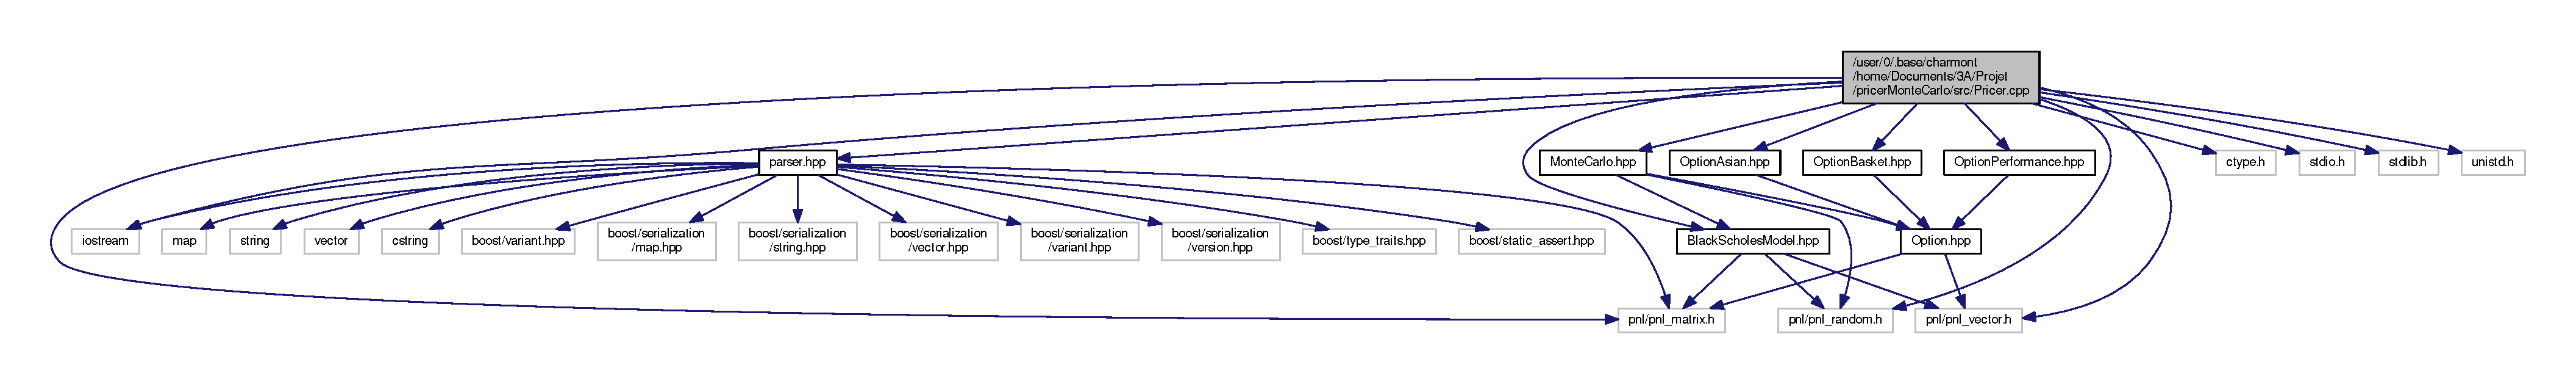
\includegraphics[width=350pt]{Pricer_8cpp__incl}
\end{center}
\end{figure}
\subsection*{Functions}
\begin{DoxyCompactItemize}
\item 
int \hyperlink{Pricer_8cpp_a3c04138a5bfe5d72780bb7e82a18e627}{main} (int argc, char $\ast$$\ast$argv)
\end{DoxyCompactItemize}


\subsection{Function Documentation}
\hypertarget{Pricer_8cpp_a3c04138a5bfe5d72780bb7e82a18e627}{\index{Pricer.\-cpp@{Pricer.\-cpp}!main@{main}}
\index{main@{main}!Pricer.cpp@{Pricer.\-cpp}}
\subsubsection[{main}]{\setlength{\rightskip}{0pt plus 5cm}int main (
\begin{DoxyParamCaption}
\item[{int}]{argc, }
\item[{char $\ast$$\ast$}]{argv}
\end{DoxyParamCaption}
)}}\label{Pricer_8cpp_a3c04138a5bfe5d72780bb7e82a18e627}


References Monte\-Carlo\-::delta(), Param\-::extract(), Monte\-Carlo\-::hedging\-P\-And\-L(), Monte\-Carlo\-::price(), and Black\-Scholes\-Model\-::simul\-\_\-market().


%--- End generated contents ---

% Index
\newpage
\phantomsection
\addcontentsline{toc}{part}{Index}
\printindex

\end{document}
